\documentclass[12pt]{article}
\usepackage[T1]{fontenc}
\usepackage{calc}
\usepackage{setspace}
\usepackage{multicol}
\usepackage{fancyheadings}

\usepackage{graphicx}
\usepackage{color}
\usepackage{rotating}
\usepackage{harvard}
\usepackage{aer}
\usepackage{aertt}
\usepackage{verbatim}

\setlength{\voffset}{0in}
\setlength{\topmargin}{0pt}
\setlength{\hoffset}{0pt}
\setlength{\oddsidemargin}{0pt}
\setlength{\headheight}{0pt}
\setlength{\headsep}{.4in}
\setlength{\marginparsep}{0pt}
\setlength{\marginparwidth}{0pt}
\setlength{\marginparpush}{0pt}
\setlength{\footskip}{.1in}
\setlength{\textwidth}{6.5in}
\setlength{\textheight}{8.5in}
\setlength{\parskip}{0pc}

\renewcommand{\baselinestretch}{1.5}

\newcommand{\bi}{\begin{itemize}}
\newcommand{\ei}{\end{itemize}}
\newcommand{\be}{\begin{enumerate}}
\newcommand{\ee}{\end{enumerate}}
\newcommand{\bd}{\begin{description}}
\newcommand{\ed}{\end{description}}
\newcommand{\prbf}[1]{\textbf{#1}}
\newcommand{\prit}[1]{\textit{#1}}
\newcommand{\beq}{\begin{equation}}
\newcommand{\eeq}{\end{equation}}
\newcommand{\bdm}{\begin{displaymath}}
\newcommand{\edm}{\end{displaymath}}
\newcommand{\script}[1]{\begin{cal}#1\end{cal}}
\newcommand{\citee}[1]{\citename{#1} (\citeyear{#1})}
\newcommand{\h}[1]{\hat{#1}}
\newcommand{\ds}{\displaystyle}

\newcommand{\app}
{
\appendix
}

\newcommand{\appsection}[1]
{
\let\oldthesection\thesection
\renewcommand{\thesection}{Appendix \oldthesection}
\section{#1}\let\thesection\oldthesection
\renewcommand{\theequation}{\thesection\arabic{equation}}
\setcounter{equation}{0}
}

\pagestyle{fancyplain}
\lhead{}
\chead{Empirical Significance of Learning with Firm-Specific Capital}
\rhead{\thepage}
\lfoot{}
\cfoot{}
\rfoot{}

\begin{document}

\begin{titlepage}
\begin{singlespace}
\title{Empirical Significance of Learning in a New Keynesian Model with Firm-Specific Capital\footnote{I am grateful for the advice and guidance of Eric Leeper, Kim Huynh, Brian Peterson, and Todd Walker; for useful conversations with Pedro Falc\~{a}o de Araujo, James Bullard, Troy Davig, Kenneth Kasa, Fabio Milani, Michael Plante, and Bruce Preston; and for comments by the participants of the 2007 Federal Reserve Bank of St. Louis Learning Week Conference, the 2007 Missouri Economics Conference and Indiana University economics department seminars.  All errors are my own.}}
\date{September 30, 2008}
\author{James Murray\\
Dahl School of Business\\
Viterbo University\footnote{\textit{Mailing address}: 900 Viterbo Drive, La Crosse, WI  54601. \textit{E-mail address}: jmmurray@viterbo.edu.  \textit{Phone number}: (608)738-5408. }}

\maketitle

\thispagestyle{empty}

\abstract{This paper examines the empirical significance of learning, a type of adaptive, boundedly rational expectations, in the U.S. economy within the framework of the New Keynesian model with endogenous capital accumulation.  Estimation results for learning models can be sensitive to the choice for agents' initial expectations, so three methods for choosing initial expectations are examined.  Maximum likelihood results show that learning under all methods do not significantly improve the fit the model.  The evolution of forecast errors show that the learning models do not out perform the rational expectations model during the run-up of inflation in the 1970s and the subsequent decline in the 1980s, a period of U.S. history which others have suggested learning may play a role.  Despite the failure of learning models to better explain the data, analysis of the impulse response functions and paths of structural shocks during the sample show that learning can lead to different explanations for the data.} \newline 

\noindent \textit{Keywords}: Learning, firm-specific capital, New Keynesian model, maximum likelihood. \\
\noindent \textit{JEL classification}: C13, E22, E31, E50.
\end{singlespace}
\end{titlepage}
\newpage

\section{Introduction}
Rational expectations is one of the most common assumptions in dynamic macroeconomic models.  While it is usually made for mathematical convenience, the assumption regarding expectations formation can have non-trivial effects on a model's dynamics.  In particular, a large amount of literature has addressed the implications of least squares learning for popular dynamic stochastic general equilibrium (DSGE) models.  Agents in a DSGE model that learn do not know the parameters of the model, and instead form expectations by collecting past data and compute least squares forecasts.  In this paper I investigate statistical evidence for learning within the framework of a New Keynesian monetary model and examine the implications of incorporating learning on the predictions of the model

Recent papers have found that least squares learning can have important effects on output and inflation determination.  \citee{ow2005} use an estimated two equation monetary model and demonstrate with simulations of impulse response functions that least squares learning can lead to prolonged inflation following an inflation shock.  Using the same model, \citee{ow2005b} find in another paper that learning on the part of monetary policy can possibly explain the period of stagflation during the 1970s.  They suggest that the monetary authority was under-estimating the natural rate of unemployment during this time, and was therefore responding too aggressively to unemployment and not enough to inflation.  They suggest that had the central bank responded to inflation instead of unemployment, lower inflation and unemployment would have resulted.  \citee{primiceri2006} suggests that learning on the part of the central bank can explain both the run-up of inflation during the 1970s and the subsequent decline during the 1980s.  He suggests that the monetary authority was under-estimating both the natural rate of unemployment and the degree of inflation persistence.  Like \citee{ow2005b}, he shows the resulting monetary policy leads to an increase in inflation, but as time progresses the central bank's expectations evolve.  The central bank's expectations of the natural rate of unemployment and the degree of inflation persistence return their actual values and therefore the policy prescription becomes stabilizing, resulting in the moderation that occurred from the middle 1980s onward.

The results from these papers depend on a calibrated value for the constant learning gain, a parameter that is responsible for the speed in which expectations evolve, and therefore responsible for the impact learning can have on the dynamics of the model.  \citee{milani2007} is the first paper to estimate the learning gain jointly with the parameters of a model.  He finds an estimate for the learning gain which is very close to calibrated values that are popular in the literature.  He estimates a standard three equation New Keynesian model and finds evidence in U.S. data that learning explains persistence in output and inflation better than habit formation and inflation indexation.  Like the papers cited above, \citename{milani2007} makes specific assumptions about the initial conditions of agents expectations.  Many of the initial conditions are set close to pre-sample ordinary least squares estimates.  The exceptions are the degree of inflation persistence, which he assumes is equal to zero, and the sensitivity of output to inflation, which he assumes is higher than the pre-sample evidence.  

The results of all of these studies depend on the assumptions for the initial conditions for agents and/or central bank's expectations.  These initial conditions are sometimes backed by an economic justification or an argument that such a set of initial conditions accounts well for the data.  In this paper, instead of suggesting a specific assumption for the initial expectations of agents, I examine a number of alternative methods for forming these initial conditions.  These methods include using the rational expectations solution of the model and using least-squares estimation results from pre-sample data.

I extend the analysis of the existing empirical learning literature, and incorporate learning into a New Keynesian model with firm-specific capital and endogenous investment decisions, a model introduced by \citee{woodford2005}.  There are a number of motivations for extending the empirical analysis to the model with capital accumulation.  Including capital in the model introduces data on another variable, aggregate investment, to be included in the estimation procedure.  Secondly, introducing capital may alter how expectations are formed, since agents may use past data on capital to make their forecasts.  Also, incorporating capital introduces more expectations into the model which may allow learning may play a bigger role.  Finally, in a rich model with stochastic shocks to preferences, technology, and investment, one can determine the role learning has on the impact of such shocks, and the role the shocks play in explaining U.S. data.

Rational expectations and learning versions of the model are estimated by maximum likelihood.  The findings of this paper indicate the learning gain is statistically significant which implies rejection of the null hypothesis of rational expectations and statistical evidence that expectations are adaptive.  Examination of the other parameter estimates indicate that allowing for learning in the model can lead agents' consumption and investment decisions to be less dependent on expectations.  Furthermore, estimated impulse response functions indicate that learning can lead to very different effects for the structural shocks depending on the information agents use for forming their forecasts and depending on the initial conditions for agents expectations at the beginning of the sample period.  Despite these differences, examination of in-sample and out-of-sample forecast errors find that the learning models do not out-perform the rational expectations model in explaining the data.

The paper is organized as follows.  Section 2 describes the details of the New Keynesian model with firm-specific capital.  Section 3 describes the learning process and how learning is incorporated into the model.  Section 4 describes the maximum likelihood procedure and the four cases for how initial conditions are constructed.  Section 5 reports the results, and section 6 concludes.

\section{Model}
The New Keynesian model has been used extensively in monetary economics for analysis of theoretical and empirical issues and it is a convenient framework to examine the role of learning on output, consumption, investment, and inflation determination.  \citee{woodford2003} provides a complete exposition of the model's micro-foundations, its many extensions, and implications for monetary policy.  The model used in this paper is an extension of the standard three equation New Keynesian suggested by \citee{woodford2005} that incorporates endogenous investment decisions in a framework of firm-specific capital, where output is produced under constant returns using labor and firm-specific capital.  Not only is firm-specific capital a more realistic assumption than a perfect rental market for capital, Woodford shows that allowing for firm-specific capital alters the coefficient on marginal cost in the Phillips curve in such a way that allows for greater price flexibility to be consistent with very small values of the coefficient, which is often seen in empirical work.  

The model has a continuum of consumers types on the unit interval, and a continuum of intermediate goods producers on the unit interval, each producing a unique intermediate good.  Each consumer type possesses a specific labor skill that can only be hired by a corresponding intermediate goods producer.  It is assumed that there are many consumers in each consumer type so that consumers do not have market power over the wage.  Production of intermediate goods also depend on capital goods which are firm-specific.  Since a capital good in firm $i$ cannot be used by another firm $j$, there is not a perfect capital rental market which would equalize the marginal product of capital across intermediate goods firms.  Therefore each firm's labor demand and pricing decision will depend on its current capital stock, which in turn depends on the firm's entire past history.

All the intermediate goods are used to produce a single type of final good, but they are imperfect substitutes for each other in production; therefore intermediate goods producing firms are monopolistically competitive.  Prices of intermediate goods are imperfectly flexible according to Calvo's (\citeyear{calvo1983}) pricing mechanism where a constant fraction of firms is able to re-optimize its price every period, and the firms selected to do so is randomly determined, independently of firms' histories or characteristics.  This setup for sticky prices may seem unrealistic, but \citee{roberts1995} shows in a model without firm-specific capital that quadratic price adjustment cost, an alternative pricing friction suggested by \citee{rotemberg1982}, yields the same solution as \citename{calvo1983} pricing.  The same is not true with firm-specific capital.  Under \citename{calvo1983} pricing, at any point in time, each firm will have a different pricing history and therefore a different capital stock.  Each firm's relative capital stock will in turn affect the pricing decision.  Under quadratic price adjustment costs, all firms face the same friction every period, and so all firms' price, labor, and investment decisions remain identical throughout time.  Therefore, even though \citename{calvo1983} pricing may seem to be an unrealistic setting, it is a convenient framework to incorporate the realistic assumption of firm heterogeneity.

\subsection{Consumers}
Each consumer type has a specific labor skill that can only be hired by a specific intermediate goods producing firm.  Since each intermediate goods firm has a different labor demand, wage income will be different for each consumer type.  Given a perfect asset market, though, consumption will be equal across all consumers.  Each consumer type $i \in (0,1)$ maximizes utility,
\beq \label{eq2:util} E_0 \sum_{t=0}^{\infty} \beta^t \left[ \frac{1}{1-\frac{1}{\sigma}} \xi_t \left(c_t - \eta c_{t-1}\right)^{1-\frac{1}{\sigma}} - \frac{1}{1+\mu} \mu_t n_t(i)^{1+\mu} \right], \eeq
subject to the budget constraint,
\beq \label{eq2:bc} c_t + b_t(i) = \frac{1+r_{t-1}}{1+\pi_t} b_{t-1}(i) + \frac{w_t(i)}{p_t} n_t(i) + \Pi_t - \tau_t \eeq
where $c_t$, consumption at time $t$, is not indexed by individual type $i$ since it is equal across all agents, $\xi_t$ is an aggregate preference shock, $n_t(i)$ and $w_t(i)/p_t$ are the labor supply and real wage of individual $i$ at time $t$, respectively, $\mu_t$ is an aggregate labor supply shock, $b_t(i)$ is individual $i$'s purchase of real government bonds at time $t$, $r_t$ is the nominal interest rate paid on government bonds, $\pi_t$ is the inflation rate, $\Pi_t$ is the value of profits earned by owning stock in firms, and $\tau_t$ is the value of real lump sum taxes.  The preference parameters are $\sigma \in (0,\infty)$, which is the pseudo intertemporal-elasticity of substitution,\footnote{When there is no habit formation and labor supply is fixed, $\sigma$ is exactly equal to the intertemporal elasticity of substitution.} $\eta \in [0,1)$, which is the degree of habit formation, and $\mu \in (0,\infty)$ which is the inverse of the elasticity of labor supply.  The appendix shows that the first order conditions for the consumer lead to the log-linear Euler equation,
\beq \label{eq2:lneuler} \h{\lambda}_{t} = E_t \h{\lambda}_{t+1} + \h{r}_t - E_t \pi_{t+1}, \eeq
where a hat indicates the percentage deviation of the variable from its steady state.\footnote{A hat is omitted from inflation because, as demonstrated in the appendix, in order to derive the Phillips curve it is necessary to assume the steady state inflation rate is equal to zero.}  Here, $\h{\lambda}_t$ is the marginal utility of real income, given by,
\beq \label{eq2:lnlambda} \h{\lambda}_t = \frac{1}{\sigma (1-\beta \eta)(1-\eta)}\left[ \beta \eta E_t \h{c}_{t+1} - (1+\beta \eta^2) \h{c}_t + \eta \h{c}_{t-1} \right] + \left(\h{\xi}_t - \beta \eta E_t \h{\xi}_{t+1} \right). \eeq
I assume that the preference shock, $\h{\xi}_t$, follows the exogenous autoregressive process,
\beq \label{eq2:xi} \h{\xi}_t = \rho_{\xi} \h{\xi}_{t-1} + \epsilon_{\xi,t}, \eeq
where $\epsilon_{\xi,t}$ is independently and identically with mean zero and variance given by $\sigma_{\xi}^2$.

When there is no habit formation, equations (\ref{eq2:lneuler}) and (\ref{eq2:lnlambda}) lead to the standard IS equation,
\bdm \h{c}_t = E_t \h{c}_{t+1} - \sigma \left( \h{r}_t - E_t \pi_{t+1} \right) + \h{\xi}_t. \edm
Habit formation is added to the model, because as equation (\ref{eq2:lnlambda}) demonstrates, habit formation introduces a source of persistence that does not depend on learning.  The larger is the degree of habit formation, the more current period marginal utility depends on past consumption.  Since consumption is related to output in the market clearing condition, habit formation creates output persistence.  Moreover, \citee{fuhrer2000} finds that habit formation leads to ``hump shaped'' impulse response functions, a phenomenon evident in the data.

\subsection{Producers}
There is one final good used for consumption and investment which is sold in a perfectly competitive market and produced with a continuum of intermediate goods.  The production function is given by,
\beq \label{eq2:yprod} y_t = \left[ \int_0^1 y_t(i)^{\frac{\theta-1}{\theta}} di \right]^{\frac{\theta}{\theta-1}} \eeq
where $y_t$ is the output of the final good, $y_t(i)$ is intermediate good $i$, and $\theta \in (1,\infty)$ is the elasticity of substitution in production.  Profit maximization leads to the demand for each intermediate good,
\beq \label{eq2:yi} y_t(i) = \left[ \frac{p_t(i)}{p_t} \right]^{-\theta} y_t, \eeq
where $p_t(i)$ is the price of intermediate good $i$ and $p_t$ is the price of the final good.  Substituting equation (\ref{eq2:yi}) into (\ref{eq2:yprod}) leads to a consumption price index that holds in equilibrium,
\beq p_t = \left[ \int_0^1 p_t(i)^{1-\theta} di \right]^{\frac{1}{1-\theta}}. \eeq

\subsubsection{Intermediate goods}
The intermediate good is produced with labor and a unique type of capital good according to the constant returns to scale production function,
\beq \label{eq2:yiprod} y_t(i) = z_t k_t(i)^{\alpha} n_t(i)^{1-\alpha} \eeq
where $k_t(i)$ is capital hired by firm $i$.  For a given level of output, intermediate goods firms choose labor demand and rent capital to minimize real total cost,
\beq \label{eq2:tckn} C_t = \frac{w_t(i)}{p_t} n_t(i) + \rho_t(i) k_t(i), \eeq
where $\rho_t(i)$ is the rental price of capital good $i$.  Log-linearizing the production function and summing over all intermediate goods firms leads to the log-linear aggregate production function,
\beq \label{eq2:lnprod} \h{y}_t = \h{z}_t + \alpha \h{k}_t + (1-\alpha) \h{n}_t. \eeq 
 
The appendix shows when firms hire optimal amounts of labor and capital, the average marginal cost among all the intermediate goods firms (in terms of the percentage deviation from the steady state) is given by,
\beq \label{eq2:mc} \h{s}_t = \frac{\alpha + \mu}{1-\alpha} \h{y}_t - \frac{\alpha(\mu+1)}{1-\alpha} \h{k}_t - \h{\lambda}_t - \frac{\mu+1}{1-\alpha} \h{z}_t, \eeq
where $\h{k}_t$ is the percentage deviation of the aggregate capital stock from its steady state.  The technology shock is assumed to follow the exogenous stochastic process,
\beq \label{eq2:zshock} \h{z}_t = \rho_z \h{z}_{t-1} + \epsilon_{z,t}, \eeq
where $\epsilon_{z,t}$ is independently and identically distributed with mean zero and variance given by $\sigma_z^2$.

\subsubsection{Firm-specific capital goods}
Capital goods firms maintain firm-specific capital stocks and rent the capital to the corresponding intermediate goods firm at a real price of $\rho_t(i)$ per unit of capital.  This assumption in not essential and is purely used for notational convenience.  This model supposes that the market for firm-specific capital is purely competitive, even though firm-specific capital cannot be sold to other firms.  This assumption assures an optimal amount of investment in each firm-specific capital good which would be the same outcome if the intermediate goods firms were to invest and own the capital themselves instead of renting it.

Capital goods firms purchase the final good and convert it to a firm-specific capital good.  The conversion from a final good to a firm-specific capital good is irreversible and is subject to a stochastic shock, $\iota_t$, that is common to all capital goods.  Let $I_t(i)$ denote the purchase of the final good for investment for capital good $i$, so that $\iota_t I_t(i)$ be the amount a purchase of $I_t(i)$ adds to the capital stock.  The evolution of firm-specific capital $i$ is given as,
\beq \label{eq2:evcap} k_{t+1}(i) = (1-\delta) k_t(i) + \iota_t I_t(i) - \frac{\phi}{2} \left[\frac{k_{t+1}(i)}{k_t(i)} - 1 \right]^2 k_t(i) \eeq
where $\delta \in (0,1)$ is the capital depreciation rate and $\phi \in (0,\infty)$ is a capital adjustment cost parameter.  When $\phi=0$, there is no adjustment cost and capital net of depreciation increases by $\iota_t I_t(i)$.  Log-linearizing equation (\ref{eq2:evcap}) then integrating across all the firms leads to the following relationship between capital and investment:
\beq \label{eq2:inv} \h{k}_{t+1} = (1-\delta)\h{k}_t + \delta \h{I}_t + \delta \h{\iota}_t \eeq

Capital goods firms choose investment to maximize the expected utility value of profits,
\beq \label{eq2:kprofit} E_0 \sum_{t=0}^{\infty} \beta^t \lambda_t \left[\rho_t(i) k_t(i) - I_t(i)\right], \eeq
subject to equation (\ref{eq2:evcap}).  The appendix shows that profit maximization leads to the following evolution of the aggregate capital stock:
\beq \label{eq2:lneqk} \begin{array}{l}
\ds \h{\lambda}_t + \phi \left(\h{k}_{t+1} - \h{k}_t\right) = \ds \beta (1-\delta) E_t \h{\lambda}_{t+1} + \left(\frac{1-\beta \left(1-\delta \right)}{1-\alpha} \right) \left[ (\mu+1) E_t \h{y}_{t+1} - (1 + \mu \alpha) \h{k}_{t+1}\right] \\ \\ 
\ds + \beta \phi \left(E_t\h{k}_{t+2} - \h{k}_{t+1}\right) - \frac{\left(\mu+1\right) \left[ 1-\beta \left(1-\delta \right) \right]}{1-\alpha} E_t \h{z}_{t+1} + \h{\iota_t} - \beta(1-\delta)E_t \h{\iota}_{t+1} \\
\ds + \left[1-\beta(1-\delta)\right] E_t \h{\mu}_{t+1}, 
\end{array} \eeq
The investment shock is assumed to follow the stochastic process,
\beq \label{eq2:mushock} \h{\iota}_t = \rho_{\iota} \h{\iota}_{t-1} + \epsilon_{\iota,t} \eeq
where $\epsilon_{\iota,t}$ is independently and identically distributed with mean zero and variance given by $\sigma_{\iota}^2$.

\subsubsection{Phillips Curve}
The Phillips curve is a single equation that describes the relationship between inflation and output, as determined by the supply side of the economy when prices are sticky.  The specific price friction employed in this paper is \citee{calvo1983} pricing.  According to this method, only a random subset of intermediate goods firms are able to re-optimize their price in a given period.  Allowing for inflation indexation, those firms who are not able to re-optimize their price may adjust their price by a fraction, $\gamma$, of the previous period's inflation rate.  Let $\omega \in (0,1)$ denote the fraction of firms who are not able to change their prices each period.  Since the specific firms able to change their prices each period is randomly determined, $\omega^T$ is the probability a firm will not be able to change its price for $T$ consecutive periods.  A firm who is able to change its price maximizes the following present discounted utility value of profits earned while the firm is unable to change its price again:
\beq \label{eq2:intprofit}
E_t \sum_{T=0}^{\infty} \left(\omega \beta \right)^{T} \frac{\lambda_{t+T}}{\lambda_t}
\left\{ \left(\frac{p_{t+T}(i)}{p_{t+T}}\right) y_{t+T}(i) - S\left[y_{t+T}(i)\right] \right\},
\eeq
where $S\left[y_{t+T}(i)\right]$ is the real total cost function of producing $y_{t+T}(i)$ units, given optimal decisions for labor and capital, and $p_{t+T}(i)$ is the firm's price in period $t+T$, given the firm has not yet been able to re-optimize its price.  When there is a positive degree of inflation indexation, this price is determined by,
\beq \label{eq2:index} \log p_{t+T}(i) = \log p_{t+T-1}(i) + \gamma \pi_{t+T-1} \eeq

The appendix shows that the firms' optimal choices for prices in combination with equilibrium in the firm-specific capital goods market leads to the following Phillips curve,
\beq \label{eq2:phillips} \pi_t = \left( \frac{1}{1+\beta \gamma} \right) \left( \gamma \pi_{t-1} + \beta E_t \pi_{t+1} + \kappa \h{s}_t \right) \eeq
where $\kappa$ decreases as $\omega$, the degree of price stickiness, increases.  The parameter $\kappa$ is also a function of other parameters of the model, but there is not a closed form expression for it.  The appendix describes the full details of the derivation of the Phillips curve.

\subsubsection{Monetary Policy}
The nominal interest rate is determined jointly with output and inflation by monetary policy.  In this paper I assume the monetary authority follows a \citee{taylor1993} type rule where the interest rate is set in response to expected output and inflation, with a preference for interest rate smoothing, according to,
\beq \label{eq2:taylor} \h{r}_t = \rho_r \h{r}_{t-1} + (1-\rho_r) \left(\psi_{\pi} E_t \pi_{t+1} + \psi_y E_t \h{y}_{t+1} \right) + \epsilon_{r,t} \eeq
where $\rho_r \in [0,1)$ is a degree of interest rate smoothing desired by the monetary authority, $\psi_{\pi} \in (0,\infty)$ is the feedback on the interest rate to expected inflation, $\psi_y \in (0,\infty)$ is the feedback on the interest rate to expected output, and $\epsilon_{r,t}$ is an independently and identically distributed exogenous monetary policy shock with mean zero and variance given by $\sigma_r^2$.  

Alternative policy rules may replace expected inflation and output with current or lagged realizations.  \citee{mccallum1997}, for example, argues that a policy rule that depends on current realizations of output and inflation is not operational.  He suggests that using lagged realizations more accurately represent actual monetary policy since current quarter estimates for output and price levels are not available.  Under rational expectations with full information, the policy rule above is also subject to this criticism.  However, as will be seen in the next section, under learning expectations are formed by collecting past data, so the monetary policy rule above is operational.

\subsection{Complete Model}
The complete system has nine variables: consumption ($\h{c}_t$), marginal utility of income ($\h{\lambda}_t$), investment ($\h{I}_t$), capital stock ($\h{k}_t$), marginal cost ($\h{s}_t$), output ($\h{y}_t$), labor ($\h{n}_t$), inflation ($\pi_t$), and the interest rate ($\h{r}_t$).   The demand side of the model consists of the Euler equation, (\ref{eq2:lneuler}), and the definition of the marginal utility of income, (\ref{eq2:lnlambda}).  The supply side of the model consists of the Phillips curve, (\ref{eq2:phillips}), the definition of the marginal cost, (\ref{eq2:mc}), the evolution of capital, (\ref{eq2:lneqk}), the relationship between investment and capital, (\ref{eq2:inv}), and the production function (\ref{eq2:lnprod}).  The model is completed with the monetary policy rule, (\ref{eq2:taylor}), and the following log-linear goods market clearing condition,
\beq \label{eq2:lnmkt} \h{y}_t = c_y \h{c}_t + \delta k_y \h{I}_t, \eeq
where $c_y$ is the steady state consumption to output ratio and $k_y$ is the steady state capital to output ratio.  The appendix shows that $k_y$ and $c_y$ are given by,
\bdm k_y = \frac{\beta \alpha (\theta-1)}{\theta \left(1 - \beta + \beta \delta\right)}, \edm
\bdm c_y = 1 - \delta k_y. \edm

There are five exogenous shocks in the model: the preference shock, $\xi_t$, whose evolution is given in equation (\ref{eq2:xi}); the technology shock, $z_t$, whose evolution is given in equation (\ref{eq2:zshock}); the investment shock, $\iota_t$, whose evolution is given in equation (\ref{eq2:mushock}); the labor supply shock, $\mu_t$, and the monetary policy shock, $\epsilon_{r,t}$.   

\section{Learning}

The specific type of adaptive learning process considered in this paper is least squares learning.  Under least squares learning, agents form expectations by collecting past data and computing least squares estimates.  The specific type of least squares learning I use is constant gain learning, which is consistent with agents' forecasts based on weighted least squares, where more recent observations are given more weight, and the weights decline geometrically with the age of the observations.  This is a popular assumption in the learning literature and is the same type of learning used by \citee{ow2005} to explain inflation scares, \citee{primiceri2006} to explain the inflation volatility in the 1970s, and \citee{milani2007} to explain output and inflation persistence.  

Constant gain least squares learning is arguably similar to how expectations are actually formed in the U.S economy.  Least squares forecasts out-perform more complex economic models in out-of-sample forecasts, and the welfare of individuals who make output, consumption, and savings decisions depend on the accuracy of forecasts and not the ability to identify parameters of an econometric model, or the ability to make counter-factual predictions.  These latter qualities, found in structural economic models, are desirable mostly by policy makers.  The constant gain assumption can also be argued as realistic as it captures the idea that agents agents believe changes in the economy are possible, so that agents view more recent data as more likely to yield accurate forecasts than data from further in the past.  I demonstrate in the next section that constant gain least squares is equivalent to a very specific type of weighted least squares which is not an actual popular estimation method.  However, \citee{evanshonka2001} suggest that constant gain least squares is a good approximation for agents that use a ``rolling window'' of data.  That is, agents do not use all the data as far back as possible, but form forecasts based on the most recent data for a given number of observations.  This is very close to common practice, as empirical studies that forecast output and inflation typically use at most 50 years of data, despite annual data available from \citee{johnstonwilliamson2007} for both these variables dating all they way back to the year 1790.

There is also a theoretical and empirical appeal to using constant gain learning.  The theoretical appeal is that unlike with ordinary least squares, with weighted least squares the effects of learning persist in the long run.  With ordinary least squares, as time progresses agents obtain more and more observations and so their sample sizes approach infinity.  Therefore, the effect a single new observation has on the agents' estimation results disappears.  Constant gain learning instead assumes that a new observation carries the same weight every period, regardless of how much time has progressed.  The empirical appeal is that the degree to which learning affects the dynamics of the economy can be determined by estimating a single parameter, the learning gain.  Moreover, with appropriate initial conditions for the learning process, constant gain learning nests the rational expectations framework, where rational expectations is the special case where the learning gain is equal to zero.  Standard statistical tests that determine if a parameter is significantly different from zero can determine the statistical significance of learning, and formally reject or fail to reject the rational expectations hypothesis.

The log-linearized New Keynesian model in the previous section has the following general form:
\beq \label{eq2:sform} \Omega_{0} x_t = \Omega_{1} x_{t-1} + \Omega_{2} E_t^* x_{t+1} + \Psi v_t, \eeq
\beq \label{eq2:sformw} v_t = A v_{t-1} + \epsilon_t \eeq
where $x_t$ is a vector of state variables (expressed as percentage deviations from their steady state), $E_t^*$ refers to a possibly non-rational expectations operator, $v_t$ is a vector of structural shocks, and $\epsilon_t$ is a vector of independently and identically distributed innovations to the shock process.  In the New Keynesian model with firm-specific capital the state vector is given by, $x_t' = [\h{y}_t~ \h{c}_t~ \h{k}_t~ \h{\lambda}_t~ \h{I}_t~ \h{n}_t~ \h{s}_t~ \pi_t~ \h{r}_t]$, and the vector of shocks is given by, $v_t = [\h{z}_t~ \h{\iota}_t~ \h{\xi}_t~ \h{\mu}_t~ \epsilon_{r,t}]$

The solution of the model can be written as,
\beq \label{eq2:msvsol} x_t = G x_{t-1} + H v_t. \eeq
To agents that learn with a correctly specified model, the actual values in the matrices $G$ and $H$ are unknown, but agents use the form of equation (\ref{eq2:msvsol}) to estimate future values of $x_t$ by least squares.  It is assumed that when agents begin period $t$, time $t$ observations are not yet realized; therefore agents collect observations up through time period $t-1$.  From this agents make least squares forecast, then make consumption, production, investment, and pricing decisions based on these expectations.  Only after these decisions are implemented, that is at the end of time period $t$, do time $t$ observations become available.  This is both a realistic and mathematically simplifying assumption.  The latest numbers from statistical agencies such as the Bureau of Labor Statistics are almost always at least one quarter old.  It is of great mathematical convenience, because the term $E_t^* x_{t+1}$ in equation (\ref{eq2:sform}) is then only a function of observations through period $t-1$.  Therefore, solving for $x_t$ in terms of past state variables is straightforward.  If instead $E_t^* x_{t+1}$ was a function of $x_t$, non-linear numerical methods would be needed to solve the model as least squares forecasts are non-linear.

To forecast $x_{t+1}$, agents estimate $G$ and $H$ by least squares using as regressors variables in the vector $x_{t-1}$, and the shocks included in $v_t$.  Assuming agents have data available on shocks is not very realistic, but this assumption can be dropped.  In Section \ref{s:estimation} I estimate the models under both cases, so that when comparing the results from the learning and rational expectations models, it will be clear what results derive from the learning process, and what results derive from assuming that agents have a more limited information set.

Agents do not use all the variables in $x_t$ as regressors, only those that correspond to non-zero columns in $G$.  If an entire column in $G$ is equal to zero, this implies that the past observation in the associated element in $x_{t-1}$ does not influence $x_t$ in the rational expectations solution.  I assume agents know the structural form of the economy and therefore use as explanatory variables only the variables that have non-zero coefficients in $G$.  In the New Keynesian model, the variables with non-zero coefficients in $G$ include consumption, capital, the inflation rate, and the interest rate.  The remaining variables in the model that are not used as explanatory variables are output, labor, marginal cost, marginal utility of income, and investment.  

I assume agents also use a constant term in their least squares forecasts.  The structural form of the model, (\ref{eq2:sform}), does not include a constant, but since this equation is written in terms of percentage deviations from the steady state, using a constant in agents' estimation equations implies agents do not know the steady state values of the economy.

Let $\Phi_t$ denote the time $t$ estimate of the all the coefficients to be estimated in the learning process.  These coefficients include a vector of constants, the non-zero columns in $G$, and all the columns in $H$ in the case where shocks are used as explanatory variables.  Let $Y_t$ denote the time $t$ dependent variables used in the learning process.  Since time $t$ data is not available to agents, $Y_t = x_{t-1}$.  Let $X_t$ denote the vector of time $t$ explanatory variables.  If agents include the stochastic shocks in their explanatory variables, $X_t' = [1~ x_{t-2}'~ v_{t-1}']$, otherwise $X_t' = [1~ x_{t-2}']$.  If agents estimate equation (\ref{eq2:msvsol}) by ordinary least squares, they form the estimate,
\beq \label{eq2:Phi} \Phi_t' = \left( \frac{1}{t-1} \sum_{\tau=2}^{t} X_{\tau} X_{\tau}' \right)^{-1} \left( \frac{1}{t-1} \sum_{\tau=2}^{t} X_{\tau} Y_{\tau}' \right). \eeq 

The ordinary least squares estimate $\Phi_t$ can be rewritten into the convenient recursive form:
\beq \label{eq2:lnPhi} \Phi_t = \Phi_{t-1} + g_t (Y_{t} - \Phi_{t-1} X_{t}) X_{t}' R_t^{-1} ,\eeq
\beq \label{eq2:lnR} R_t = R_{t-1} + g_t (X_{t} X_{t}' - R_{t-1}), \eeq
where $g_t=1/(t-1)$ is the learning gain.\footnote{To show this, let $R_t = \frac{1}{t-1} \sum_{\tau=2}^{t} X_{\tau} X_{\tau}'$ and $\Phi' = R_t^{-1} \left( \frac{1}{t-1} \sum_{\tau=2}^{t} X_{\tau} Y_{\tau}' \right)$}  The recursive form demonstrates precisely how expectations are adaptive.  Agents take the previous period's estimates, $\Phi_{t-1}$ and $R_{t-1}$, and correct them according to the residual between the previous period's forecast and the new observation.  The amount of the correction depends on the learning gain.  With ordinary least squares and infinite memory, the learning gain approaches zero as time approaches infinity, so the effect new observations have on updating the beliefs of $\Phi$ and $R$ diminish as the number of observations already in the sample approaches infinity.  Constant gain learning instead assumes that the learning gain $g_t$ remains constant over time.  This allows new observations to influence estimation results by the same weight throughout time.  If the constant gain is equal to zero, the estimate $\Phi_t$ remains at its initial value throughout time.  Given an initial value equal to the rational expectations solution, a zero constant learning gain implies rational expectations.

Let $\h{g}_{0,t}$ denote the estimated constant term in $\Phi_t$, and let $\h{G}_t$ and $\h{H}_t$ denote the time $t$ estimate of $G$ and $H$, respectively, obtained from $\Phi_t$.  Agents' expectation of $x_{t+1}$ is given by, 
\beq \label{eq2:agfore} E_t^* x_{t+1} = \h{g}_{0,t} + \h{G}_t E_t^* x_t + \h{H} E_t v_{t+1} \eeq
Note that equation (\ref{eq2:agfore}) assumes that expectations about future shocks, $v_{t+1}$, are rational.  This is a common simplifying assumption made in learning models.  It is possible to allow agents to also estimate the coefficients in the shock process, but the dynamics deriving from this additional complication are negligible.  Since time $t$ observations are not yet available to agents, agents must also estimate $x_t$ by least squares.  The time $t$ estimate of $x_t$ is given by,
\beq \label{eq2:agfore1} E_t x_t^* = \h{g}_{0,t} + \h{G}_t x_{t-1} + \h{H}_t v_t. \eeq
Plugging this into equation (\ref{eq2:agfore}) yields,
\beq \label{eq2:agfore2} E_t^* x_{t+1} = (I + \h{G}_t)\h{g}_{0,t} + \h{G}_t^2 x_{t-1} + \left(\h{G}_t \h{H}_t + \h{H}_t A \right) v_t. \eeq

Plugging the agents' forecast, (\ref{eq2:agfore2}), into the structural form of the model, (\ref{eq2:sform}), leads to the following actual law of motion for $x_t$:
\beq \label{eq2:alm} x_t = \Omega_0^{-1}\Omega_{2}\left(I+\h{G}_t\right)\h{g}_{0,t} + \Omega_0^{-1} \left(\Omega_{1} + \Omega_{2} \h{G}_t^2 \right) x_{t-1}  + \Omega_0^{-1} \left[ \Psi + \Omega_2 \left(\h{G}_t \h{H}_t + \h{H}_t A \right) \right] v_t. \eeq

\section{Estimation}\label{s:estimation}
\subsection{Data}
I estimate the model with quarterly U.S. data on real private consumption, real gross private domestic investment, consumer price index inflation, and the effective federal funds rate.  Data is collected for 1970:Q1 through 2008:Q1 from the Federal Reserve Bank of St. Louis FRED database.  Consumption and investment are put in per-capita terms by dividing the series by data on the civilian non-institutional population which is obtained from the Bureau of Labor Statistics.

In the New Keynesian model, consumption and investment are expressed in terms of the percentage deviation from their respective steady states.  Since this data is non-stationary it is first de-trended by removing a common trend growth rate, similar to \citename{ireland2004} \citeyear{ireland2004} and \citeyear{ireland_tech_2004}.  Even though productivity growth is not specified in the model, consumption and investment should have the same long run growth rate.  This growth rate is determined by adding together consumption and investment, and taking the average growth rate over the sample.  The average quarterly growth rate of output computed this way is $g_y = 0.0054$.  De-trended consumption and investment is therefore determined according to,
\bdm CONS_t^* = \frac{CONS_t}{\left(1+g_y\right)^t}, \mbox{           } INV_t^* = \frac{INV_t}{\left(1+g_y\right)^t}, \edm
where $CONS_t$ and $INV_t$ are the raw data on consumption and investment, and $CONS_t^*$ and $INV_t^*$ denote the data with the trend growth rate removed.

\subsection{Initial conditions}
I estimate the model under four different cases for how expectations are formed.  Case 1 is rational expectations, and the other cases are learning with different assumptions for initial expectations and what explanatory variables agents use to make their least squares forecasts.  Case 2 can be viewed as the closest to rational expectations.  Agents learn according to constant gain least squares, but the initial values for the learning matrices $\Phi$ and $R$ are equal to the rational expectations solution.  Furthermore, agents have the same information as agents with rational expectations, which means they include realizations of structural shocks among the other explanatory variables.  When the constant learning gain is equal to zero, Case 2 is equivalent to Case 1.   

Case 3 makes another incremental step away from rational expectations.  Agents again learn according to constant gain least squares, and their initial conditions for the learning matrices are equal to the rational expectations values, but agents are not able to collect data on past shocks in order to use them as explanatory variables.  

Case 4 assumes the agents have the same information set as Case 3, but the initial conditions for the learning process matrices are different from the rational expectations solution.  The initial conditions are set equal to constant gain least squares estimates from pre-sample data.  This is similar to how \citee{milani2007} initializes the learning matrices, but he uses estimates from a first order vector autoregression using ordinary least squares, which is consistent instead with a decreasing learning gain.  In this paper, the initial conditions for the learning process are consistent with the constant learning gain which is estimated jointly with the other parameters of the model.

Equations (\ref{eq2:lnPhi}) and (\ref{eq2:lnR}) describe the least squares learning process with any given learning gain, $g_t$.  When the learning gain is constant, repeated substitution of these equations can show that the coefficient matrix is given by,
\beq \label{eq2:Phisum} \Phi_t = \left( \sum_{\tau=0}^{t-1} \left(1-g\right)^t X_{t-\tau} X_{t-\tau}' \right)^{-1} \left( \sum_{\tau=0}^{t-1} \left(1-g\right)^t X_{t-\tau} Y_{t-\tau}' \right) \eeq

In the New Keynesian model with firm-specific capital, $Y_t' = [\h{c}_{t-1}~ \h{k}_{t-1}~ \pi_{t-1}~ \h{r}_{t-1}]$, and $X_t' = [1~ \h{c}_{t-2}~ ~\h{k}_{t-2}~ \pi_{t-2}~ \h{r}_{t-2}]$.  In this specification of the model, some of the data agents use are not directly observed by the econometrician.  Consumption is expressed as percentage deviations from the steady state, and capital stock is not directly observable.  For a given estimate of the consumption to output ratio and the steady state level of output, pre-sample data on aggregate consumption is put in terms of the percentage deviation from the steady state according to,
\beq \label{eq2:cinit} \h{c}_t = \frac{CONS_t^* - c_y y^*}{c_y y^*}, \eeq
where $c_y$ is the steady consumption to output ratio, one of the New Keynesian model parameters to be estimated, and $y^*$ is the steady state level of output which will be calibrated, as discussed in the next subsection.

The inflation rate is directly observable by the econometrician, but to make solving the New Keynesian model tractable, it was assumed in Section 2 that the steady state inflation rate is equal to zero.  Since this is unlikely to be the case in the data, let $\pi^*$ denote the annualized steady state inflation rate, expressed as a percentage.  Let $INF_t$ denote the annualized quarterly inflation rate measured from CPI data.  This data is mapped to pre-sample data for $\pi_t$ according to,
\beq \label{eq2:piinit} \pi_t = \frac{1}{400}\left(INF_t - \pi^*\right). \eeq
The steady state inflation rate, $\pi^*$, will also be calibrated as discussed in the next section.

The interest rate in the model is also expressed as a deviation from its steady state.  The steady state real gross interest rate in the New Keynesian model is given by $\beta^{-1}$.  Let $r^*$ denote the annualized quarterly steady state interest rate so that $r^*=400(\beta^{-1}-1)$.  Let $FF_t$ denote data on the annualized quarterly federal funds Rate.  Pre-sample data on the federal funds rate can therefore be transformed to pre-sample data for agents according to
\beq \label{eq2:rinit} \h{r}_t = \frac{1}{400}\left(FF_t - r^* - \pi^*\right). \eeq

Data for the U.S. capital stock is difficult to measure, but using the New Keynesian model, data for percentage deviation of capital from its steady state level can be composed from data on the deviation of investment from its steady state level.  Recall equation (\ref{eq2:inv}) describes the evolution of the capital stock in terms of the percentage deviation from the steady state:
\beq \label{eq2:kinit} \h{k}_{t+1} = (1-\delta)\h{k}_t + \delta \h{I}_t + \delta \h{\iota}_t. \eeq
For a given initial value for $\h{k}_t$ in the pre-sample, a simulated path for the investment shock, $\h{\iota}_t$, and pre-sample data on the percentage deviation of investment from the steady state, $\h{I}_t$, a pre-sample series of $\h{k_t}$ can be constructed.  Investment in the model is expressed as a percentage deviation from its steady state.  Similar to consumption data, pre-sample data on gross private domestic investment can be transformed to pre-sample data for $\h{I}_t$ according to,
\beq \label{eq2:invinit} \h{I}_t = \frac{INV_t^* - (1-c_y) y^*}{(1-c_y) y^*}, \eeq
where $(1-c_y)y^*$ is the steady state level of investment.

I suppose at the beginning of the pre-sample capital is equal to its steady state value so that the pre-sample initial value for $\h{k}_t$ is set equal to zero.  The investment shock series is generated equation (\ref{eq2:mushock}) given the variance of the investment shock, $\sigma_{\iota}^2$, which is estimated along with the rest of the parameters of the model in the maximum likelihood procedure.  

Pre-sample quarterly data is collected for 1954:Q3 through 1969:Q4 and is transformed to pre-sample data for $\h{c}_t$, $\h{k}_t$, $\pi_t$, and $\h{r}_t$ according to equations (\ref{eq2:cinit}), (\ref{eq2:piinit}), (\ref{eq2:rinit}), (\ref{eq2:kinit}), (\ref{eq2:mushock}), and (\ref{eq2:invinit}).  The initial condition for $\Phi_0$ is then computed using equation for the weighted least squares procedure, equation (\ref{eq2:Phisum}).

\subsection{Maximum Likelihood Procedure}
I estimate the model by maximum likelihood following the Kalman filter procedure outlined in chapter 13 of \citee{hamilton}.  This procedure involves rewriting the model into state space form.  The state equation is a linear equation describing the entire New Keynesian model including the learning mechanism.  The equations governing the state are the actual law of motion for $x_t$, given in equation (\ref{eq2:alm}), and the evolution of the structural shocks given in equation (\ref{eq2:sformw}).  Equation (\ref{eq2:alm}) can be rewritten more compactly as,
\beq \label{eq2:almFM} x_t = b_t + F_t x_{t-1} + M_t v_t, \eeq
where vector $b_t$ and matrices $F_t$ and $M_t$ are given by,
\bdm b_t = \Omega_0^{-1}\Omega_{2}\left(I+\h{G}_t\right)\h{g}_{0,t}, \edm
\bdm F_t = \Omega_0^{-1} \left(\Omega_{1} + \Omega_{2} \h{G}_t^2 \right), \edm
\bdm M_t = \Omega_0^{-1} \left[ \Psi + \Omega_2 \left(\h{G}_t \h{H}_t + \h{H}_t A \right) \right] \edm

This equation can be combined with equation (\ref{eq2:sformw}) into the single state equation,
\beq \label{eq2:state} x_t^* = b_t^* + F_t^* x_{t-1}^* + \epsilon_t^*, \eeq
where $x_t^* = [x_t'~ v_t']'$ and, 
\bdm F_t^* = \left[ \begin{array}{cc} F_t & M_t A \\ 0 & A \end{array} \right], \edm
\bdm b_t^* = \left[ \begin{array}{c} b_t \\ 0 \end{array} \right], \edm
\bdm \epsilon_t^* = \left[ \begin{array}{c} M_t \epsilon_t \\ \epsilon_t \end{array} \right]. \edm
The variance of $\epsilon_t^*$ is given by,
\bdm \label{eq2:Q} Var(\epsilon_t^*) = \left[ \begin{array}{cc} M_t \Sigma M_t' & M_t \Sigma \\ \Sigma M_t' & \Sigma \end{array} \right], \edm
where $\Sigma$ is a diagonal matrix with the variance of the structural shocks along the diagonal.

The observations equations are given by,
\beq \begin{array}{c} CONS_t^* = c_y y^* + c_y y^* \h{c}_t \\ 
                      INV_t^* = (1-c_y) y^* + (1-c_y) y^* \h{I}_t \\ 
		      INF_t = \pi^* + 400 \pi_t \\ 
		      FF_t = \pi^* + 400 \left(r^n + \h{r}_t\right), \end{array} \eeq

The likelihood is maximized with respect to the following vector of parameters,
\bdm \Theta_2 = [\eta~ \sigma~ \mu~ c_y~ \phi~ \gamma~ \rho_r~ \psi_y~ \psi_{\pi}~ \rho_z~ \rho_{\iota}~ \rho_{\xi}~ \sigma_z~ \sigma_{\iota}~ \sigma_{\xi}~ \sigma_r~ g]. \edm
Several parameters are calibrated instead of estimated.  The discount factor, $\beta$, is set equal to $0.9925$ which corresponds to a steady state real interest rate approximately equal to 3\%.  The depreciation rate, $\delta$, is set equal to $0.025$ which corresponds to an approximate annual depreciation rate of 10\%.

The steady state level of inflation, $\pi^*$, is set equal to $3.67$, the average inflation rate over the entire pre-sample and sample period.  The steady state level of output $y^*$ is set equal to the average of $CONS_t^* + INV_t^*$ over the sample and pre-sample period, which is computed to be $y^*=14,355$.  This is the average de-trended estimate for real per-capita output, when considering only investment and consumption and ignoring other spending that contributes to real GDP such as government spending and net exports. 

Preliminary estimation results led to unreasonably low values for $\kappa$, the slope on the Phillips curve that depends on the degree of price flexibility, and $\alpha$, the capital-share of income.  \citee{ireland_tech_2004} also reports difficulty in obtaining sensible estimates for the Phillips curve slope using maximum likelihood, calibrates this parameter to $\kappa=0.1$.  \citee{smetswouters2005} in very rich New Keynesian with capital accumulation report difficulty in estimating the capital-share of income and calibrate it to $\alpha=0.24$.  I follow each of these papers and use the calibrations.

Finally, data on total hours of labor is not used in the estimation procedure, so the labor supply shock $\h{\mu}_t$ is suppressed, which leaves $\rho_{\mu}$ and $\sigma_{\mu}$ out of the estimation.

\section{Results}
\subsection{Parameter Estimates}
The parameter estimates for the four cases for expectations formation are given in Table \ref{tb2:parms}.  In this subsection I look at each case in turn. \\

\noindent \textbf{Case 1: Rational Expectations}

The first two columns of Table \ref{tb2:parms} show the parameter results for rational expectations.  The parameter estimates for the sources of persistence are markedly low.  The estimate for degree of habit formation is $\eta=0.1060$, the estimate for the degree of price indexation is $\gamma=0.3624$, and the estimate of the degree of monetary policy persistence is $\rho_r=0.1945$.  These are quite small compared to much of the empirical literature for dynamic macroeconomic models.  For example, for U.S. data, \citee{smetswouters2005} find a degree of habit formation equal to $0.69$ and a degree of price indexation equal to $0.66$.  \citee{milani2007} also predicts significant degrees for these sources of persistence, but only when estimating his model under rational expectations.  

Some empirical work finds similar evidence for weak sources of persistence.  \citee{ireland_tech_2004} estimates by maximum likelihood a three equation New Keynesian model that is augmented with sources of persistence for output and inflation and finds estimates of these parameters statistically insignificantly different from zero.  \citee{csb2005} estimate the Phillips curve side of the model and find a median estimate for the degree of inflation indexation equal to zero.  Despite the weak evidence for persistence from habit formation and price indexation, the persistence in the structural shocks in the model are all very significant.  All these estimates are in excess of $0.9$, and strongly significantly different from zero.

The estimated intertemporal elasticity of substitution is approximately equal to $\sigma=0.1603$, which is rather small compared to other findings.  For example, \citee{smetswouters2005} estimate the inverse elasticity equal to $1.62$, implying the elasticity is approximately $0.61$.  \citee{giannoni_woodford_2003} find a similar estimate of $0.66$.  The estimate of this parameter may depend crucially on the assumed expectations mechanism since it measures the response of current period consumption decisions to changes in the expected real interest rate.  This matter is further examined with Cases 2, 3 and 4 below.

The point estimate for the inverse elasticity of labor supply is approximately $\mu=30.67$ which implies labor supply is very inelastic.  One place in the model this parameter enters is in the evolution of capital stock implied by the optimal investment decision, given in equation (\ref{eq2:lneqk}).  This equation illustrates that large values for $\mu$ imply relatively small responses in $k_{t+1}$, and therefore current period's optimal choice for investment, to changes in expectations for future output and future technology shocks.  Due to the relationship of this parameter and expectations, the estimate of this parameter is also possibly dependent on the assumed expectations mechanism.

The estimate for the cost of capital adjustment is equal to $7.68$.  This is relatively close to the finding in \citee{smetswouters2005} and the calibration used in \citee{woodford2005}.  Dividing every term in equation (\ref{eq2:lneqk}) illustrates that this parameter also measures how responsive investment decisions are to changes in expectations.  The larger is the cost of adjusting capital, the less responsive is investment to changes in expected output, expected technology shocks, and expected investment shocks. 

Finally the monetary policy parameters indicate a strong response of the Federal Funds rate to expected inflation, $\psi_{\pi}=2.1212$, and virtually no response to the deviation of expected output from its steady state, $\psi_{y}=0.0000$.  The more than one-to-one response of the Federal Funds rate to inflation is a common finding in the literature using data during the Volcker-Greenspan period after 1982.  \citee{ls2004} find evidence that the response was smaller before this period, but since the sample period for this paper begins in 1970, most of the sample is data from a period where U.S. monetary policy is widely viewed as aggressively targeting inflation to promote macroeconomic stability.  The absent response to output is somewhat different than what is found in the literature.  \citee{smetswouters2005} use a more rich specification for the Taylor rule and find a similar weak response to current output, but a stronger response to lagged output.  \\

\noindent \textbf{Case 2: Learning with RE Initial Conditions}

The next two columns of Table \ref{tb2:parms} show the results for learning when agents expectations at the beginning of the sample are set equal to the rational expectations solution, and agents use data on all the shocks to form their expectations, which is the same information set for rational expectations.  Rational expectations is the special case when the learning gain, $g$, is equal to zero.  

The point estimate for the learning gain for Case 2 is $0.0240$ and is statistically significantly different from zero, which implies significant statistical evidence to reject the null hypothesis that expectations are rational.  This is close to commonly calibrated values in the learning literature, for example \citee{primiceri2006} uses a calibration equal to $0.015$ and \citee{ow2005} uses a value of $0.05$.  This is also very close to Milani's (\citeyear{milani2007}) estimate of $0.018$.

While constant gain learning implies that agents use weighted least squares with a possibly indefinitely large sample, \citee{evanshonka2001} and \citee{sargent1999} among others have suggested that constant gain learning should closely resemble learning with ordinary least squares in which agents use a rolling window of approximately $1/g$ observations, since the additional weight given to a new observation in such a framework is also constant and equal to $g$.  With this interpretation of the learning gain, the parameter estimate implies that agents look at data from the last 41.6 quarters, or almost 10.5 years.

Three parameter estimates, those for the intertemporal elasticity of substitution ($\sigma$), the inverse elasticity of labor supply ($\mu$), and the cost of capital adjustment ($\phi$), are very different from Case 1.  All these parameters move in the direction that causes consumption and investment decisions to be less responsive to changes in expectations.  The estimate for the intertemporal elasticity of substitution is approximately $\sigma=0.0513$ which is about one third the size of the estimate under rational expectations.  This implies that learning leads to the prediction that consumption decisions are less responsive to changes in the expected real interest rate.  

The estimate for the inverse elasticity of labor supply is $\mu=0.0499$, markedly different from the estimate under rational expectations.  This implies a very elastic labor supply, and therefore a much smaller response in investment decisions to changes in expected future output and technology shocks.  The direction for this different finding is intuitive.  Given the finding that learning models predict agents decisions are less responsive to changes in expectations, changes in investment decisions will be less responsive if labor supply is elastic, since then firms can respond by changing their hiring decisions with relatively small changes in the real wage.

The estimated cost of capital adjustment is approximately $\phi=24.8826$, much higher than predicted by rational expectations.  Since adjusting capital is relatively more expensive, investment decisions are less responsive to changes in expectations about output, technology shocks, and investment shocks.

Finally, this learning framework implies a lesser monetary policy response to expected inflation, and a larger response to expected output.  The finding that monetary policy is more responsive to output in the learning framework is related to \citee{smetswouters2005} finding that monetary policy responds more to lagged output than concurrent output.  \citee{mccallum1997} also argues that it is more realistic to suppose the monetary authority only has information on lagged output.  Under learning, agents collect information up through the previous period, therefore expectations of future output depend completely on past data of output, not on current realizations. \\

\noindent \textbf{Case 3: Learning with RE Initial Conditions and Unobservable Shocks}

The next two columns of Table {\ref{tb2:parms} show the estimation results when agents learn, but with a more limited information set than Cases 1 and 2.  In Case 3 agents do not collect data on past realizations of structural shocks to use for explanatory variables in their forecasts.  For the first period in the sample, the coefficients on the remaining explanatory variables are initialized to the rational expectations solution.

The estimate for the learning gain is approximately $0.0236$ and is again statistically significantly different from zero.  This does not imply a formal rejection of rational expectations as before, since the rational expectations framework is no longer a special case, but it does imply statistical evidence that expectations are adaptive.  The estimate for the learning gain implies that agents use approximately 42.4 past quarters of data to form their expectations, or about 10.5 years. 

Some notable differences in the estimates from the previous expectations frameworks again include the intertemporal elasticity of substitution, the inverse elasticity of labor supply, and cost of adjusting capital.  The intertemporal elasticity of substitution is even smaller than the previous two cases, which means this framework for learning predicts an even smaller response of consumption decisions to changes in the expected real interest rate.  

The estimate for the inverse of labor supply is $\mu=2.0877$ which implies labor is inelastic.  This is still far below the estimate under rational expectations, but much larger than the estimate under the learning framework in case 2.  Therefore when not supposing that agents observe structural shocks to form their expectations, investment decisions are more sensitive to changes in expected future output relative to when agents do collect data on structural shocks.  When agents only use past data on observable macroeconomic variables, current period shocks have no influence on expectations, so agents forecasts should be less volatile.  Given a less volatile series for expectations, it is expected that an equivalent change in expectations should have a larger impact on agents' decisions than with more volatile expectations that is predicted when agents do observe shocks.  Such an explanation is consistent with the larger estimate for $\mu$, but possibly contradicts the finding that the estimate for $\sigma$ is smaller.  The estimate for the standard deviation of the preference shock is much higher in Case 3 than Cases 1 and 2.  This causes consumption decisions to be more volatile which likely influences the estimate for the intertemporal elasticity of substitution.

The estimate for the cost of adjusting capital is approximately $\phi=26.83$, which is not significantly different than under case 2, but still significantly greater than the estimate under rational expectations. \\

\noindent \textbf{Case 4: Learning with Pre-Sample Initial Conditions}

The final learning framework assumes agents have the same information set as Case 3, but initial conditions for the learning matrices are set equal to weighted least squares estimates obtained from pre-sample data.  The estimate for the learning gain is approximately $g=0.0381$, which is slightly larger than the previous estimates.  This again suggests statistical evidence than expectations are adaptive.  This estimate implies that agents use approximately 26.25 quarters, or about 6.5 years, of past data to form their forecasts.

The estimate for the elasticity of substitution is approximately $\sigma=0.1220$ which is not very different than predicted under rational expectations.  However, the estimate for elasticity of labor supply and cost of adjusting capital tell a similar story as Case 2.  Relative to rational expectations, this framework for learning implies investment decisions are much less responsive to changes in expectations for future output.

\subsection{Performance Comparison}
The top part of Table \ref{tb2:rmse} reports the in-sample root mean squared error (RMSE) of the residuals, that is the one-period ahead forecast errors for consumption, investment, inflation, and the federal funds rate.  The table shows no clear improvement in performance by including learning in the model.  The expectations framework that best described consumption and inflation is the learning model with observable shocks. The framework that best describes investment is the learning model with unobservable shocks.  The framework that best describes the federal funds rate is rational expectations, yet the RMSE for the federal funds rate is very close across the first three cases.  Case 4, learning with initial expectations based on pre-sample data, is the worst performing model for consumption, investment, and the federal funds rate; and is the second worst performing model for the inflation rate. 

The bottom part of Table \ref{tb2:rmse} shows the first-order autocorrelation for the squared residuals.  If the New Keynesian model is correctly specified, and accurately captures the run-up of macroeconomic volatility in the 1970s and the subsequent decline after 1982, one would expect no autocorrelation in the residuals.  Cases 1, 2, and 3 show autocorrelation insignificantly different from zero for the volatility in consumption and investment residuals.  This suggests the New Keynesian model with firm-specific capital can adequately explain the dynamics of these variables under learning or rational expectations.  However, in Cases 1, 2, and 3, the autocorrelation for the volatility in the inflation rate and federal funds rate residuals are significantly positive, which implies the models do not accurately capture the changing volatility in the data for inflation or monetary policy.  

These results flip for Case 4.  Here there is insignificant autocorrelation in the volatility for inflation and the federal funds rate residuals, but a higher degree of autocorrelation for the volatility of consumption and investment residuals.  

To better understand the relative performance of each expectations framework over the sample period, Figure \ref{fg2:fe} shows the plots the each series of forecast errors.  Periods of recession in U.S. history are shaded.  The number in parentheses is the correlation of the series of forecast errors of the respective learning model with the series predicted under rational expectations.  The forecast errors for all four variables for Cases 2 and 3 are highly correlated with rational expectations.  The largest forecast errors are made during the 1970s and early 1980s, a period many agree was marked by excessive macroeconomic volatility.  The largest forecast errors for the federal funds rate are made just after 1980 when Paul Volcker became chairman of the Federal Reserve and began to aggressively counter-act very high levels of inflation.

 The forecast errors under Case 4 are significantly less correlated with the rational expectations case, but it tells the same qualitative story.  The model makes the largest forecast errors for consumption, investment, and inflation during the 1970s and early 1980s.

To get a further understanding of the relative performance of each model I next examine how they compare in out-of-sample extended forecasts.  To do this I first estimate the model using the sub-sample 1970:Q1 through 1989:Q4, then use this set of parameters to make out-of-sample extended forecasts for forecast horizons 1 period ahead through 12 periods ahead for the remainder of the sample, 1990:Q1 through 2008:Q1.  Figure \ref{fg2:rmse} shows the RMSE's for consumption, investment, inflation and the federal funds rate for each of the four expectations frameworks.  The horizontal axis is the forecast horizon and the vertical axis is the root mean squared error.  The vertical axis is logarithmic in order for the RMSE's for each expectations framework to show nicely on each graph.

The results from Figure \ref{fg2:rmse} show the rational expectations model performs nearly as well out-of-sample as most of the learning models.  The worst performing model for investment, inflation, and the federal funds rate is Case 2, the learning model arguably closest to rational expectations.  Recall, in this framework agents include data on structural shocks to form their forecasts, and expectations at the beginning of the sample are set equal to the rational expectations solution.  In this framework the learning matrices, $\Phi_t$ and $R_t$ evolve with realizations of the shock processes.  Under rational expectations, agents expectations also depend on structural shocks, but the learning matrices are constant throughout time, equal to the rational expectations solution.  Out-of-sample forecasts for the structural shocks generate imprecise forecasts for the learning matrices, and therefore poor out-of-sample forecasts.  This result would not be expected for a learning gain very close to zero.  If the learning gain were very small, the learning gain matrices would be very slow to evolve.  

\subsection{Structural Shocks}
Despite the similar performance of the four models for in-sample and out-of-sample forecast errors, the choice for how expectations are formed makes a difference for predictions for the structural shocks.  Figures \ref{fg2:irf_pref}, \ref{fg2:irf_tech}, \ref{fg2:irf_inv}, and \ref{fg2:irf_mp} show the impulse responses to consumption, investment, inflation, and the interest rate for each shock under each of the expectations frameworks. 

Impulse responses for learning models depend on the values of the learning matrices $\Phi_t$ and $R_t$ at the time of the impulse.  The impulse response functions computed in this paper are for the state of the learning matrices at the first quarter of 2008, the last period of the sample.  If the learning matrices are not equal to the rational expectations solution, then even in the absence of shocks the state variables evolve as expectations converge to the rational expectations solution.  Therefore, to expose only the impact of the shocks, the plots in Figures \ref{fg2:irf_pref}, \ref{fg2:irf_tech}, \ref{fg2:irf_inv}, and \ref{fg2:irf_mp} show the difference between the evolution of the variables after the shock and the evolution the variables would take in the absence of any shocks.

The figures show persistent impacts on consumption, investment, and the interest rate from preference, technology, and investment shocks under rational expectations.  In Case 2 the shocks cause large, long lasting, oscillatory effects on investment, inflation, and the interest rate.  This oscillatory behavior is likely what causes the large out-of-sample forecast errors for Case 2.  The figures show when expectations are initialized based on pre-sample data (Case 4), the responses to the four shocks also cycle back and forth but are much more jagged, more volatile, but shorter lasting.

When agents do have data on structural shocks, the effects of structural shocks can have opposite impacts as when agents do observe structural shocks.  For example, the first and second rows of Figure \ref{fg2:irf_pref} show when there is a positive preference shock and agents can observe the shock, and therefore recognize that it is temporary, the interest rate increases in response to the increase in consumption and investment decreases.  In Case 3 where agents learn and do not observe the shock, the increase in consumption demand causes agents to expect permanently higher consumption and therefore increase investment.  

Figure \ref{fg2:irf_inv} shows when there is a positive investment shock, in Case 2 there is an increase in investment demand as agents expect investment to be more productive.  In Case 3, agents cannot view the shock and so do not initially expect investment to be more productive.  The shock does cause an unexpected increase in the capital stock which decreases the marginal product of capital and therefore decreases the demand for investment.  

Figure \ref{fg2:irf_mp} shows the impact of a contractionary monetary policy shock.  In Cases 1 and 2 when agents observe the monetary policy shock, the demand for consumption and investment decrease.  When agents do not observe the shock, the stochastic behavior of the interest rate causes agents to alter their expectations for the behavior of monetary policy.  The supply for output increases causing an increase in consumption and investment and a decrease in inflation.  The negative response to inflation then causes the monetary authority to actually decrease the interest rate after the initial positive shock.

To understand how these impulse responses influence the predictions of the model, Figure \ref{fg2:shocks} shows the smoothed estimates\footnote{Kalman filter smoothing is computed using the techniques described in \citee{jong1989}.} for the evolution of the structural shocks over the sample period.  Again, periods of U.S. recession are shaded and the number in parentheses is the correlation of each shock with the prediction under rational expectations.  The evolution of the preference shock under Cases 1, 2, and 3 are all very similar.  In each of these cases the preference shock is near is lowest during the 1980 and 1981 recessions.  Other than this instance, the preference shock seems to have little correlation with onset of recessions.  The same is not true for Case 4.  The preference shock under Case 4 is completely uncorrelated with the prediction under rational expectations, and shows only small dips during recessionary periods.

The evolution of the technology shocks in Cases 3 and 4 are highly correlated with the rational expectations prediction, but the Case 2 evolution of technology shocks is completely uncorrelated.  Recall from Figure \ref{fg2:irf_tech} that in Case 2, technology shocks cause long-lived oscillatory behavior in consumption, investment, and inflation, whereas under rational expectations and Case 3, the responses of these variables are in one direction and long lived.  Despite the lack of correlation in the technology shock in Case 2, all cases have a similar qualitative story.  All recessionary periods are marked by low realization of the technology shock.  The difference in Case 2 is that the drop in the technology shock actually precedes the recessions, instead of dropping during the recessions as in other cases.  In fact from 1980 through 1982 the technology shock is actually recovering in Case 2, but remaining low in all the other frameworks.

The evolution of the investment shock is very different among the four cases.  Under rational expectations, the recessions in the early 1980s are characterized by large positive investment shocks.  Recall from Figure \ref{fg2:irf_inv} that a positive investment shock under rational expectations causes a negative response to consumption and a positive response to investment, inflation, and the interest rate.  These responses are consistent with the United States experience during the late 1970s and early 1980s, a period marked by high unemployment and high inflation, and a time when the Federal Reserve began to drastically increase the federal funds rate in response to high inflation.  The same is not true for Case 2.  Figure \ref{fg2:irf_inv} shows that consumption responds positively to an investment shock, the initial positive response to investment is much larger, and the responses to investment and inflation are shorter lived.  The evolution of the investment shock therefore looks somewhat different over the sample period.  The investment shock still reaches peaks during this time, but it is not as dramatic as under rational expectations.  

The evolution of the investment shock in Cases 3 and 4 are similar to each other, but very different from Cases 1 and 2.  Here the recessions in the early 1980s are characterized by negative investment shocks.  When agents do not use structural shocks to form their expectations, Figure \ref{fg2:irf_inv} shows that positive investment shocks lead to a drop in inflation, a sustained positive response to consumption, and a fall in the interest rate.  The early 1980s were instead characterized by decreases in consumption and increases in interest rates, therefore, the investment shock falls during this period, which is the opposite of the finding in Cases 1 and 2.

\section{Conclusion}
Constant gain learning is found to not significantly out-perform rational expectations in the context of a standard Keynesian model that is extended to account for endogenous firm-specific capital accumulation.  Three different learning frameworks are examined that differ based on the initial conditions for agents' expectations and the information set available to agents when making their forecasts.  The models are estimated by maximum likelihood and the results indicate that learning provides minimal to no improvement in the fit of the model to U.S. data.  When the learning procedure is initialized using least squares estimation results from pre-sample data, the model actually performs the worst as measured by in-sample forecast errors.  Out-of-sample extended forecast errors show the worse performing model is the learning framework in which agents do have information on all structural shocks and expectations at the beginning of the sample are set equal to rational expectations.  Despite the mixed results for the fit for the various models to the data, this paper does find a constant learning gain statistically significantly different from zero in all cases, which implies statistical evidence that expectations are not rational and are adaptive.  

Impulse response functions and smoothed estimates of the structural shocks reveal that each expectations framework provides very different explanations for the impacts a structural shock can have and therefore each model predicts different evolutions for the structural shocks over the sample period.  The impulse response functions show when agents learn and have data on structural shocks, there can be long-lived oscillatory effects on consumption, investment, and inflation.  When agents do not observe the structural shocks, some of the impulse responses are reversed.  These different responses to structural shocks lead to different evolutions for the structural shocks over the sample period, especially for the technology and investment shocks.





\newpage
\nocite{*}
\bibliographystyle{econometrica}
\bibliography{learning_capital}

\newpage
\app
\section{Derivation of New Keynesian model}\label{s:apnkpc}
\subsection{Consumers}
Consumers choose consumption, $c_t$, labor supply, $n_t(i)$, and purchases of bonds, $b_t(i)$, to maximize utility, given in equation (\ref{eq2:util}), subject to the budget constraint, given in equation (\ref{eq2:bc}).  The first order conditions are,
\bdm \lambda_t = \xi_t \left(c_t - \eta c_{t-1}\right)^{-\frac{1}{\sigma}} - \beta \eta E_t \xi_{t+1} \left(c_{t+1} - \eta c_t\right)^{-\frac{1}{\sigma}} \edm
\bdm \mu_t n_t(i)^{\mu} = \lambda_t \frac{w_t(i)}{p_t} \edm
\bdm \lambda_t = \beta E_t \lambda_{t+1} \frac{1+r_t}{1+\pi_{t+1}} \edm
where $\lambda_t$ is the Lagrange multiplier for the budget constraint and therefore the marginal utility of real income.  Log-linearizing the first order conditions yields,
\beq \label{ap:lnlambda} \h{\lambda}_t = \frac{1}{\sigma (1-\beta \eta)(1-\eta)}\left[ \beta \eta E_t \h{c}_{t+1} - (1+\beta \eta^2) \h{c}_t + \eta \h{c}_{t-1} \right] + \left(\h{\xi}_t - \beta \eta E_t \h{\xi}_{t+1} \right) \eeq
\beq \label{ap:lnlabor} \h{w}_{t}(i) - \h{p}_t = \mu \h{n}_{t}(i) - \h{\lambda}_t + \h{\mu}_t\eeq 
\beq \label{ap:lneuler} \h{\lambda}_{t} = E_t \h{\lambda}_{t+1} + \h{r}_t - E_t \pi_{t+1} \eeq
where a hat indicates the percentage deviation of the variable from its steady state.  Equation (\ref{ap:lnlabor}) will be referenced later to express equilibrium real wages in terms of employment.  Equations (\ref{ap:lneuler}) and (\ref{ap:lnlambda}) together implicitly define the log-linear Euler equation which determines consumers' demand for final goods.

\subsection{Producers}
\subsubsection{Final goods firms}
The final goods firm chooses its demand for intermediate good $i$ to maximize profits,
\bdm \Pi_t = p_t \left[ \int_0^1 y_t(i)^{\frac{\theta-1}{\theta}} di \right]^{\frac{\theta}{\theta-1}} - \int_0^1 p_{t}(i) y_{t}(i) di \edm
The first order condition leads to the demand for intermediate good $i$,
\beq \label{ap:yi} y_t(i) = \left[ \frac{p_t(i)}{p_t} \right]^{-\theta} y_t. \eeq
which is given in equation (\ref{eq2:yi}).

\subsubsection{Input choices}
Intermediate goods firms choose labor demand and rent capital to minimize real total cost, given in equation (\ref{eq2:tckn}), subject to the production function, given in equation (\ref{eq2:yiprod}).  The first order conditions are,
\beq \label{ap:focn} \frac{w_t(i)}{p_t} = (1-\alpha) s_t(i) \frac{y_t(i)}{n_t(i)}, \eeq
\beq \label{ap:fock} \rho_t(i) = \alpha s_t(i) \frac{y_t(i)}{k_t(i)}, \eeq
where $s_t(i)$ is the Lagrange multiplier on the production function.  The Lagrange multiplier is interpreted as the change in the objective function from a marginal ease in the constraint.  In this case the objective function is total cost and the constraint is total output, so the Lagrange multiplier is equal to the marginal cost.

Log-linearizing the first order conditions yields,
\beq \label{ap:lnkfoc} \h{\rho}_t(i) = \h{s}_t(i) + \h{y}_t(i) - \h{k}_t(i), \eeq
\beq \label{ap:lnnfoc}\h{w}_t(i) - \h{p}_t = \h{s}_t(i) + \h{y}_t(i) - \h{n}_t(i), \eeq
Combining these two equations to eliminate $\h{s}_t(i)$ and substituting equation (\ref{ap:lnlabor}) to eliminate wages and prices leads to the expression for the rental rate of capital,
\beq \label{ap:lnrho1} \h{\rho}_t(i) = \left(\mu + 1\right) \h{n}_t(i) -\h{k}_t(i) - \h{\lambda}_t + \h{\mu}_t. \eeq
The production function can now be used to express the rental rate of capital only in terms of output and capital.  The log-linear production function is given by,
\beq \label{ap:lnyiprod} \h{y}_t(i) = \h{z}_t + \alpha \h{k}_t(i) + (1-\alpha) \h{n}_t(i). \eeq
Solving equation (\ref{ap:lnyiprod}) for $\h{n}_t(i)$ and substituting this into (\ref{ap:lnrho1}) yields,
\beq \label{ap:lnrho2} \h{\rho}_t(i) =  \frac{\mu+1}{1-\alpha} \h{y}_t(i) - \frac{1+\mu\alpha}{1-\alpha} \h{k}_t(i) - \h{\lambda}_t + \h{\mu}_t - \frac{\mu+1}{1-\alpha} \h{z}_t \eeq
Solving equation (\ref{ap:lnkfoc}) for $\h{s}_t(i)$ and using equation (\ref{ap:lnrho2}) to substitute out $\h{\rho}_t(i)$ leads to the expression for marginal cost for firm $i$,
\beq \label{ap:mci} \h{s}_t(i) = \frac{\alpha+\mu}{1-\alpha} \h{y}_t(i) - \frac{1+\alpha \mu}{1-\alpha} \h{k}_t(i) - \h{\lambda}_t + \h{\mu}_t - \frac{\mu+1}{1-\alpha} \h{z}_t \eeq
Summing over all the firms leads to the average marginal cost in the economy,
\beq \label{ap:mc} \h{s}_t = \frac{\alpha + \mu}{1-\alpha} \h{y}_t - \frac{\alpha(\mu+1)}{1-\alpha} \h{k}_t - \h{\lambda}_t + \h{\mu}_t - \frac{\mu+1}{1-\alpha} \h{z}_t \eeq
Subtracting equation (\ref{ap:mc}) from equation (\ref{ap:mci}), leads to an expression for the marginal cost of firm $i$ in terms of the average marginal cost and the firms relative output and capital stock,
\beq \label{ap:mci2} \h{s}_t(i) = \h{s}_t + \frac{\alpha+\mu}{1-\alpha} \left[\h{y}_t(i) - \h{y}_t\right] - \frac{\alpha+\mu}{1-\alpha} \tilde{k}_t(i) \eeq
where $\tilde{k}_t(i) = \h{k}_t(i) - \h{k}_t$ is the relative capital stock of firm $i$.

\subsubsection{Capital goods firms}
Capital goods firms maximize the utility value of profits, given in equation (\ref{eq2:kprofit}), subject to the evolution of firm-specific capital stock, given in equation (\ref{eq2:evcap}).  Instead of explicitly computing the profit maximizing choice of investment, one can solve the evolution of capital for $I_t(i)$ and substitute this into the objective function.  The first order condition is,
\beq \begin{array}{l} \label{ap:focI} 
\ds \frac{\lambda_t}{\iota_t} \left[1+\phi \left(\frac{k_{t+1}(i)}{k_t(i)} - 1\right)\right] = \\ \\
\ds \beta E_t \frac{\lambda_{t+1}}{\iota_{t+1}} \left[ \iota_{t+1} \rho_{t+1}(i) + (1-\delta) + \phi \left(\frac{k_{t+2}(i)}{k_{t+1}(i)} - 1\right) \frac{k_{t+2}(i)}{k_{t+1}(i)} - \frac{\phi}{2} \left(\frac{k_{t+2}(i)}{k_{t+1}(i)} - 1\right)^2 \right]. 
\end{array} \eeq
Log-linearizing this yields,
\beq \label{ap:lnifoc} \begin{array}{l} 
\ds \h{\lambda}_t + \phi \left(\h{k}_{t+1}(i) - \h{k}_t(i)\right) = E_t \h{\lambda}_{t+1} + \left[1-\beta \left(1-\delta \right) \right] E_t \h{\rho}_{t+1}(i) \\ \\
\ds + \beta \phi \left(E_t\h{k}_{t+2}(i) - \h{k}_{t+1}(i)\right) + \h{\iota}_t - \beta(1-\delta)E_t \h{\iota}_{t+1}. 
\end{array} \eeq
Plugging equation (\ref{ap:lnrho2}) into (\ref{ap:lnifoc}) leads to the following equilibrium condition for the evolution of capital stock for firm $i$:
\beq \label{ap:lneqki} \begin{array}{l}
\ds \h{\lambda}_t + \phi \left(\h{k}_{t+1}(i) - \h{k}_t(i)\right) = \ds \beta (1-\delta) E_t \h{\lambda}_{t+1} \\ \\
\ds + \left(\frac{1-\beta \left(1-\delta \right)}{1-\alpha} \right) \left[ (\mu+1) E_t \h{y}_{t+1}(i) - (1+\mu\alpha) \h{k}_{t+1}(i)\right] + \beta \phi \left(E_t\h{k}_{t+2}(i) - \h{k}_{t+1}(i)\right) \\ \\ 
\ds + \left[1-\beta(1-\delta)\right] E_t \h{\mu}_{t+1} - \frac{\left(\mu+1\right) \left[ 1-\beta \left(1-\delta \right) \right]}{1-\alpha} E_t \h{z}_{t+1} + \h{\iota}_t - \beta(1-\delta)E_t \h{\iota}_{t+1}. 
\end{array} \eeq
Integrating equation (\ref{ap:lneqki}) over all firms leads to the evolution of the aggregate capital stock,
\beq \label{ap:lneqk} \begin{array}{l}
\ds \h{\lambda}_t + \phi \left(\h{k}_{t+1} - \h{k}_t\right) = \ds \beta (1-\delta) E_t \h{\lambda}_{t+1} + \left(\frac{1-\beta \left(1-\delta \right)}{1-\alpha} \right) \left[ (\mu+1) E_t \h{y}_{t+1} - (1+\mu\alpha) \h{k}_{t+1}\right] \\ \\ 
\ds + \beta \phi \left(E_t\h{k}_{t+2} - \h{k}_{t+1}\right) - \frac{\left(\mu+1\right) \left[ 1-\beta \left(1-\delta \right) \right]}{1-\alpha} E_t \h{z}_{t+1} + \h{\iota_t} - \beta(1-\delta)E_t \h{\iota}_{t+1} \\
\ds + \left[1-\beta(1-\delta)\right] E_t \h{\mu}_{t+1}, 
\end{array} \eeq
which is shown in equation (\ref{eq2:lneqk}) of the paper.  Subtracting equation (\ref{ap:lneqk}) from equation (\ref{ap:lneqki}) leads to following expression for firm $i$'s capital stock in terms of the aggregate capital stock,
\beq \label{ap:kki} \begin{array}{l}
\ds \phi \left( \tilde{k}_{t+1}(i) - \tilde{k}_{t}(i) \right) = \beta \phi \left(E_t\tilde{k}_{t+2}(i) - \tilde{k}_{t+1}(i) \right) \\ \\
\ds + \left[ \frac{1-\beta \left(1-\delta \right)}{1-\alpha} \right] \left[ (\mu+1) E_t \left( \h{y}_{t+1}(i) -\h{y}_{t+1} \right)  - (1+\mu\alpha) \tilde{k}_{t+1}(i) \right].
\end{array} \eeq

\subsubsection{Optimal pricing}
The inflation indexation rule given in equation (\ref{eq2:index}) can be re-written so that future prices intermediate goods firms will charge while not being able to re-optimize their price can be expressed in terms of the price chosen by the firm at time $t$.  By repeated substitution of equation (\ref{eq2:index}), the price at time $t+T$ of good $i$ can be expressed as,
\bdm p_{t+T}(i) = p_t(i) \exp \left( \gamma \sum_{\tau = 0}^{T-1} \pi_{t + \tau} \right), \edm
For notational convenience, let $\pi_{t+T}^* \equiv \sum_{\tau = 0}^{T-1} \pi_{t + \tau}$.  Substitute the demand equation, (\ref{eq2:yi}), into the profit function, (\ref{eq2:intprofit}), to express the profit only in terms of the intermediate good price, $p_t(i)$, and aggregate state variables the firm cannot control:
\beq \label{ap:intprofit2}
E_t \sum_{T=0}^{\infty} \left(\omega \beta \right)^{T} \frac{\lambda_{t+T}}{\lambda_t}
\left\{ \left(\frac{p_t(i) e^{\gamma \pi_{t+T}^*}}{p_{t+T}}\right)^{1-\theta} y_{t+T} - S\left[\left(\frac{p_t(i) e^{\gamma \pi_{t+T}^*} }{p_{t+T}}\right)^{-\theta} y_{t+T} \right] \right\}.
\eeq
The first order condition with respect to $p_t(i)$ is given by,
\beq \label{ap:intfoc} E_t \sum_{T=0}^{\infty} \left(\omega \beta \right)^{T} 
\frac{\lambda_{t+T}}{\lambda_t}
\left\{ \left( 1-\theta \right) \left(\frac{p_t^*(i) e^{\gamma \pi_{t+T}^*}}{p_{t+T}}\right)^{1-\theta} 
+ \theta s_{t+T}(i) \left(\frac{p_t^*(i) e^{\gamma \pi_{t+T}^*}}{p_{t+T}}\right)^{-\theta} \right\}
\frac{y_{t+T}}{p_t^*(i)} = 0, \eeq
where $p_t^*(i)$ is the optimal price for a firm that is able to re-optimize its price.  Since the first order condition cannot be rewritten in terms of inflation instead of prices, it is necessary to assume prices have a steady state, which implies the steady state level of inflation is equal to zero.  Before log-linearizing, it is convenient to rearrange equation (\ref{ap:intfoc}) as,
\beq \label{ap:intfoc2} \begin{array}{l}
\ds \left( 1-\theta \right) E_t \sum_{T=0}^{\infty} \left(\omega \beta \right)^{T} 
\lambda_{t+T} \left(\frac{p_t^*(i) e^{\gamma \pi_{t+T}^*}}{p_{t+T}}\right)^{1-\theta} y_{t+T} = \\ \\ 
\ds - \theta E_t \sum_{T=0}^{\infty} \left(\omega \beta \right)^{T} \lambda_{t+T}
s_{t+T}(i) \left(\frac{p_t^*(i) e^{\gamma \pi_{t+T}^*}}{p_{t+T}}\right)^{-\theta} y_{t+T}, 
\end{array} \eeq
then log-linearize each side of the equal sign separately.  Log-linearizing the left hand side and right hand size, respectively, yield,
\beq \label{ap:lleft} \left(1-\theta \right) \lambda y E_t \sum_{T=0}^{\infty} 
\left(\omega \beta \right)^{T} \left[\h{\lambda}_{t+T} + \h{y}_{t+T} + 
\left(1-\theta \right) \left(\h{p}_t^*(i) - \h{p}_{t+T} + \gamma \pi_{t+T}^* \right) \right], \eeq
\beq \label{ap:lright} -\theta \lambda y s E_t \sum_{T=0}^{\infty} 
\left(\omega \beta \right)^{T} \left[\h{\lambda}_{t+T} + \h{y}_{t+T} + \h{s}_{t+T} 
-\theta \left(\h{p}_t^*(i) - \h{p}_{t+T} + \gamma \pi_{t+T}^* \right) \right] \eeq
where $\lambda$ is the steady state marginal utility of income, $y$ is the steady state level of output, and $s$ is the steady state marginal cost.  Steady state marginal utility and steady output cancel out from the left and right hand sides.  The steady state marginal cost is found by evaluating the first order condition (\ref{ap:intfoc}) where $\lambda_t = \lambda$ and $p_t^*(i)=p_t=p$ for all $t$.  In the steady state equation (\ref{ap:intfoc}) simplifies to,
\bdm \left( \frac{1}{1-\omega \beta} \right) \frac{\left(1-\theta+\theta s\right)y}{p} = 0.\edm
The steady state solution for $s$ is given by,
\beq \label{ap:sss} s = -\frac{1-\theta}{\theta}. \eeq
The coefficient $-\theta~s$ in equation (\ref{ap:lright}) therefore cancels out with $1-\theta$ in equation (\ref{ap:lleft}).  Combining the left and right hand side then yields,
\beq E_t \sum_{T=0}^{\infty} \left(\omega \beta \right)^{T} \left[\h{p}_t^*(i) - \h{p}_{t+T} + \gamma \pi_{t+T}^* - \h{s}_{t+T}(i) \right] = 0 \eeq
Solving for $\h{p}_t^*(i)$ yields,
\beq \label{ap:ptisum} \h{p}_t^*(i) = \left(1-\omega \beta \right)E_t \sum_{T=0}^{\infty} \left(\omega \beta \right)^{T} \left[\h{p}_{t+T} - \gamma \pi_{t+T}^* + \h{s}_{t+T}(i) \right]. \eeq
Substitute into equation (\ref{ap:ptisum}), the log-linearized the demand for intermediate good $i$ at time $t+T$, which is given by,
\beq \label{ap:lyidem} \h{y}_{t+T}(i)=-\theta (\h{p}_t^*(i) - \h{p}_{t+T} + \gamma \pi_{t+T}^*) + \h{y}_{t+T} \eeq
and the marginal cost given in equation (\ref{ap:mci2}).  This leads to an expression for the optimal price for firm $i$ in terms of aggregate variables and the firm's expected future capital,
\beq \label{ap:ptisol} \begin{array}{ll}
\ds \h{p}_t^*(i) = & 
\ds \left(1-\omega \beta \right)E_t \sum_{T=0}^{\infty} \left(\omega \beta \right)^{T} \left\{ \h{p}_{t+T} - \gamma \pi_{t+T}^* + \h{s}_{t+T} -\frac{\theta \left(\alpha + \mu \right)}{1-\alpha} \left[\h{p}_t^*(i) - \h{p}_{t+T} + \gamma \pi_{t+T}^* \right] \right\} \\ \\ 
 & \ds - \left(1-\omega \beta \right)E_t \sum_{T=0}^{\infty} \left(\omega \beta \right)^{T} \left\{ \frac{\alpha \left(\mu+1 \right)}{1-\alpha} \tilde{k}_{t+T}(i) \right\}. 
\end{array} \eeq
The solution of this equation for $\h{p}_t^*(i)$ is given by,
\beq \label{ap:ptisumk} \h{p}_t^*(i) = \left( 1-\omega \beta \right) E_t \sum_{T=0}^{\infty} \left(\omega \beta \right)^{T} \left[ \h{p}_{t+T} - \gamma \pi_{t+T}^* + \psi \h{s}_{t+T} - \frac{\psi \alpha (\mu+1)}{1-\alpha} \tilde{k}_{t+T}(i) \right], \eeq 
where 
\bdm \psi = \left[1+\frac{\theta(\alpha + \mu)}{1-\alpha} \right]^{-1}. \edm
Equation (\ref{ap:ptisumk}) can be rewritten as the first order difference equation:
\beq \label{ap:ptistar} \h{p}_t^*(i) = \omega \beta E_t \h{p}_{t+1}^*(i) + (1-\omega \beta) \left( \h{p}_t + \psi \h{s}_t - \frac{\psi \alpha (\mu+1)}{\mu(1-\alpha)} \tilde{k}_t(i) \right), \eeq
where $E_t \h{p}_{t+1}^*(i)$ denotes the expectation at time $t$ for the time $t+1$ optimal decision for the firm's new price, conditional that the firm is able to re-optimize its price again in period $t+1$.  Note, this is not the same as the unconditional time $t$ expectation of the firm's price in period $t+1$.  Since with probability $\omega$ the firm will not be able to re-optimize its price next period, the unconditional expectation for firm $i$'s price in period $t+1$ is given by,
\beq \label{ap:Eprel} E_t \h{p}_{t+1}(i) = \omega \left[ \h{p}_t^*(i) + \gamma \pi_{t-1} \right] + (1-\omega) E_t \h{p}_{t+1}^*(i). \eeq

\subsubsection{Phillips Curve Solution}
Deriving the Phillips curve when there is firm-specific capital is substantially more complicated than a model without capital or with a perfect capital rental market.  Equation (\ref{ap:ptistar}) shows that each firm's optimal price will depend on its capital stock relative to the aggregate capital stock.  Since a firm's capital stock is dependent on its entire investment history, the optimal price will depend on the firm's entire history of being able to re-optimize its price.  The convenient result from the previous section that each firm will choose the same price does not hold when there is firm-specific capital and \citename{calvo1983} pricing.  

Equation (\ref{ap:ptisol}) implicitly defines the optimal choice for the price of intermediate good $i$ in terms of expectations of aggregate variables and the following expectation of the firm's future relative capital stocks:
\beq \label{ap:ksum} E_t \sum_{T=0}^{\infty} \left(\omega \beta \right)^{T} \tilde{k}_{t+T}(i) \eeq
To derive the Phillips curve, we must rewrite the above expression in terms of the firm's current capital stock, the current optimal price, and expectations of aggregate variables.  The optimal choice for $\tilde{k}_{t+1}(i)$ in terms of expected future output is given in equation (\ref{ap:kki}).  Substituting the log-linear demand for $y_{t+1}(i)$ into equation (\ref{ap:kki}) leads to,
\beq \label{ap:kkip} \begin{array}{l}
\ds \phi \left( \tilde{k}_{t+1}(i) - \tilde{k}_{t}(i) \right) = \beta \phi \left(E_t\tilde{k}_{t+2}(i) - \tilde{k}_{t+1}(i) \right) \\ \\
\ds - \left[ \frac{1-\beta \left(1-\delta \right)}{1-\alpha} \right] \left[ \theta (\mu+1) E_t \tilde{p}_{t+1}(i) - (1 + \mu \alpha) \tilde{k}_{t+1}(i) \right].
\end{array} \eeq
where $\tilde{p}_{t+1}(i) = \h{p}_{t+1}(i) - \h{p}_{t+1}$ is the relative price of intermediate good $i$ in period $t+1$.  The rational expectations solution for (\ref{ap:kkip}) must have the form,
\beq \label{ap:kmn} \tilde{k}_{t+1}(i) = m \tilde{k}_{t}(i) + n \tilde{p}_t(i), \eeq
where $m$ and $n$ are determined by the method of undetermined coefficients in the next subsection.  For a firm re-optimizing their price, this equation can be rewritten as
\beq \label{ap:ktilde_mn} \tilde{k}_{t+1}(i) = m \tilde{k}_{t}(i) + n \h{p}_t^*(i) - n \h{p}_t(i). \eeq
Substituting this into equation (\ref{ap:ksum}) shows that,
\bdm E_t \sum_{T=0}^{\infty} \left(\omega \beta \right)^{T} \tilde{k}_{t+T+1}(i) = m E_t \sum_{T=0}^{\infty} \left(\omega \beta \right)^{T} \tilde{k}_{t+T}(i) + \frac{n}{1-\omega \beta} \h{p}_t^*(i) - n E_t \sum_{T=0}^{\infty} \left(\omega \beta \right)^{T} \h{p}_{t+T}. \edm
Multiply both sides of this equation by $(\omega \beta)$ then add $\tilde{k}_t(i)$ to both sides in order to make the summation on the left hand side identical to the summation on the right hand side.  Doing this yields,
\bdm E_t \sum_{T=0}^{\infty} \left(\omega \beta \right)^{T} \tilde{k}_{t+T}(i) = \omega \beta m E_t \sum_{T=0}^{\infty} \left(\omega \beta \right)^{T} \tilde{k}_{t+T}(i) + \frac{\omega \beta n}{1-\omega \beta} \h{p}_t^*(i) - \omega \beta n E_t \sum_{T=0}^{\infty} \left(\omega \beta \right)^{T} \h{p}_{t+T} + \tilde{k}_{t}(i). \edm
Solving this equation yields,
\beq \label{ap:ksumsol} E_t \sum_{T=0}^{\infty} \left(\omega \beta \right)^{T} \tilde{k}_{t+T}(i) = \frac{1}{1-\omega \beta m} \left[ \frac{\omega \beta n}{1-\omega \beta} \h{p}_t^*(i) + \tilde{k}_t(i) - \omega \beta n E_t \sum_{T=0}^{\infty} \left(\omega \beta \right)^{T} \h{p}_{t+T} \right]. \eeq
Substituting this into equation (\ref{ap:ptisol}) and solving for $\h{p}_t^*(i)$ leads to the following solution,
\beq \label{ap:pstarsolk} \h{p}_t^*(i) = (1-\omega \beta) E_t \sum_{T=0}^{\infty} (\omega \beta)^T \left( \h{p}_{t+T} - \gamma \pi_{t+T}^* + \nu \h{s}_{t+T} \right) - \frac{\alpha \nu (\mu+1)(1-\omega \beta)}{(1-\alpha) (1-\omega \beta m)} \tilde{k}_{t}(i), \eeq
where,
\bdm \nu = \left[ 1 + \frac{\theta (\alpha + \mu)}{1-\alpha} + \frac{\alpha \omega \beta n (\mu+1)}{(1-\alpha)(1-\omega \beta m)} \right]. \edm
Equation (\ref{ap:pstarsolk}) expresses the optimal price of intermediate good $i$ solely in terms of aggregate variables and the firm's current relative capital stock.  Since the capital stock was chosen in the previous period, it is independent of whether or not a firm is currently able to re-optimize its price.  Therefore the average capital stock among firms re-optimizing their price is equal to the average capital stock in the economy.  This implies that average value for $\tilde{k}_t(i)$ over firms re-optimizing their price is equal to zero.  Let $\h{p}_t^*$ denote the average price among these firms.  Equation (\ref{ap:pstarsolk}) implies,
\beq \label{ap:pstarind} \h{p}_t^* = (1-\omega \beta) E_t \sum_{T=0}^{\infty} (\omega \beta)^T \left( \h{p}_{t+T} - \gamma \pi_{t+T}^* + \nu \h{s}_{t+T} \right). \eeq
This can be rewritten as the first order difference equation,
\beq \label{ap:pstard} \h{p}_t^* = \omega \beta E_t \h{p}_{t+1}^* + (1-\omega \beta) \left( \h{p}_t + \nu \h{s}_t \right). \eeq
Substituting equation (\ref{ap:pstarind}) into (\ref{ap:pstard}) to eliminate $\h{p}_t^*$ and $E_t \h{p}_{t+1}^*$ leads to the Phillips curve,
\beq \pi_t = \left(\frac{1}{1+\beta \gamma}\right) \left[ \gamma \pi_{t-1} + \beta E_t \pi_{t+1} + \kappa \h{s}_t \right], \eeq
where,
\bdm \kappa = \frac{(1-\omega)(1-\omega \beta)}{\nu \omega}. \edm

\subsubsection{Method of Undetermined Coefficients}
This subsection uses the method of undetermined coefficients to compute the values of $m$ and $n$ in equation (\ref{ap:ktilde_mn}) which must satisfy the optimality condition for capital given in equation (\ref{ap:kkip}).  Equation (\ref{ap:kkip}) can be rearranged as,
\beq \label{ap:ktilde1} \tilde{k}_{t+1}(i) = \tilde{k}_t(i) + \beta E_t \tilde{k}_{t+2}(i) - \zeta_0 E_t \tilde{p}_{t+1}(i) - \zeta_1 \tilde{k}_{t+1}(i), \eeq
where $\zeta_0$ and $\zeta_1$ are given by,
\bdm \zeta_0 = \frac{\theta \left(\mu+1\right) \left[1 - \beta \left( 1-\delta \right) \right]}{\phi \left(1-\alpha \right)} \edm
\bdm \zeta_1 = \beta + \frac{\left( 1+\alpha \mu \right) \left[1 - \beta \left( 1-\delta \right) \right]}{\phi \left(1-\alpha \right)} \edm

I begin by finding an expression for $E_t \tilde{p}_{t+1}(i)$ in terms of $\tilde{k}_t(i)$ and $\tilde{p}_{t}(i)$.  Using equation (\ref{ap:Eprel}), the expected relative price can be rewritten as,
\beq \label{ap:ptilde} E_t \tilde{p}_{t+1}(i) = E_t \h{p}_{t+1}(i) - E_t \h{p}_{t+1} =  \omega \h{p}_t(i) + (1-\omega) E_t \h{p}_{t+1}^*(i) - E_t \h{p}_{t+1} \eeq
In order to express $\tilde{p}_{t+1}(i)$ only in terms of $\tilde{p}_t(i)$ and $\tilde{k}_t(i)$, we must next find a solution for $\h{p}_t^*(i)$.  According to equation (\ref{ap:ptistar}), the rational expectation solution for $\h{p}_t^*(i)$ must take the form,
\beq \label{ap:pstar_a} \h{p}_{t}^*(i) = f(\h{p}_t,\h{s}_t) + a \tilde{k}_t(i), \eeq
where $f(\cdot)$ is a linear function of aggregate variables and $a$ needs to be determined by the method of undetermined coefficients.  Let $\script{L}_t$ denote the set of firms re-optimizing their price in period $t$.  The average price of the firms who are able to re-optimize their price is given by,
\bdm \h{p}_t^* = \frac{1}{1-\omega} \int_{i\in \script{L}_t} \h{p}_{t}^*(i) di = f(\h{p}_t,\h{s}_t) + \frac{a}{1-\omega} \int_{i\in \script{L}_t} \tilde{k}_t(i) di \edm
Since $\tilde{k}_t(i)$ was chosen in period $t-1$, it is independent of whether a firm is re-optimizing its price.  Therefore the average difference between a firm's capital stock and the aggregate capital stock among firms re-optimizing their price is equal to zero.  Therefore,
\bdm \h{p}_t^* = f(\h{p}_t,\h{s}_t), \edm
and equation (\ref{ap:pstar_a}) can be rewritten as,
\beq \label{ap:pstar_a1} \h{p}_t^*(i) = \h{p}_t^* + a \tilde{k}_{t}(i). \eeq
Advancing equation (\ref{ap:pstar_a1}) one period and taking expectations yields,
\beq \label{ap:Epstar1} E_t \h{p}_{t+1}^*(i) = E_t \h{p}_{t+1}^* + a \tilde{k}_{t+1}(i), \eeq
where $E_t \h{p}_{t+1}^*$ is the expected average price over firms that can re-optimize their price next period.  This can be rewritten in terms of the expected aggregate price level.  Since a fraction $\omega$ firms will not be able to change their price next period and the remaining $1-\omega$ firms will have an average price $\h{p}_{t+1}^*$, the expected price level next period is given by,
\beq \label{ap:Eptp1} E_t \h{p}_{t+1} = \omega \h{p}_t + (1-\omega) E_t \h{p}_{t+1}^*. \eeq
Solving (\ref{ap:Eptp1}) for $E_t \h{p}_{t+1}^*$ and substituting this expression into (\ref{ap:Epstar1}) leads to,
\beq \label{ap:Epstar2} E_t \h{p}_{t+1}^*(i) = \frac{1}{1-\omega} \left(E_t \h{p}_{t+1} - \omega \h{p}_t \right) + a \tilde{k}_{t+1}(i). \eeq
Substituting equation (\ref{ap:ktilde_mn}) for $\tilde{k}_{t+1}(i)$ yields,
\beq \label{ap:Epstar3} E_t \h{p}_{t+1}^*(i) = \frac{1}{1-\omega} \left(E_t \h{p}_{t+1} - \omega \h{p}_t \right) + a m \tilde{k}_{t}(i) - a n \tilde{p}_t(i). \eeq
Plugging this into equation (\ref{ap:ptilde}) leads to an expression for $E_t \tilde{p}_{t+1}(i)$ in terms of $\tilde{p}_t(i)$ and $\tilde{k}_t(i)$,
\beq \label{ap:ptilde2} E_t \tilde{p}_{t+1}(i) = \left[\omega + \left(1-\omega \right) a n\right] \tilde{p}_{t}(i) + \left(1-\omega \right) a m \tilde{k}_t(i) \eeq

Next, using equation (\ref{ap:ktilde_mn}), the expected future capital stock is given by,
\beq \label{ap:ktilde2} E_t \tilde{k}_{t+2}(i) = m^2 \tilde{k}_t(i) + m n \tilde{p}_t(i) + n E_t \tilde{p}_{t+1}(i) \eeq
Substituting equation (\ref{ap:ptilde2}) into equation (\ref{ap:ktilde2}) leads to an expression for $E_t \tilde{k}_{t+2}(i)$ in terms of $\tilde{p}_t(i)$ and $\tilde{k}_t(i)$,
\beq E_t \tilde{k}_{t+2}(i) = \left[m^2 + amn\left(1-\omega \right) \right] \tilde{k}_t(i) + \left[ mn + n\omega + a n^2(1-\omega) \right] \tilde{p}_{t}(i) \eeq
Plugging in equations (\ref{ap:ptilde2}), (\ref{ap:ktilde2}), and (\ref{ap:ktilde_mn}) into (\ref{ap:ktilde1}) leads to an expression for capital of the form given in equation (\ref{ap:ktilde_mn}) where $m$ and $n$ must satisfy, respectively,
\beq \label{ap:mcond} \beta m^2 + \left[\beta a n (1-\omega) - \zeta_1 - \zeta_0 a (1-\omega) - 1\right] m + 1 = 0, \eeq
\beq \label{ap:ncond} \beta a (1-\omega) n^2 + \left[\beta m + \beta \omega - \zeta_1 - \zeta_0 a (1-\omega) - 1\right] n - \zeta_0 \omega = 0. \eeq

All that remains is to find an expression for $a$, also using the method of undetermined coefficients.  Substituting the expression for $E_t \h{p}_{t+1}^*(i)$ given in equation (\ref{ap:Epstar3}) into equation (\ref{ap:ptistar}) and solving for $\h{p}_t^*(i)$ yields,
\beq \begin{array}{ll}
\ds \h{p}_t^*(i) = & \ds \frac{1}{1-\omega \beta a n} \left( \omega \beta a m - \frac{\psi \alpha \left(\mu + 1\right)}{(1-\alpha)} \right) \tilde{k}_{t}(i) \\ \\ 
 & \ds + \frac{\omega \beta}{\left(1-\omega \right) \left(1-\omega \beta a n \right)} \left( E_t \h{p}_{t+1} - \omega \h{p}_t \right) +  \h{p}_t + \frac{\psi}{1-\omega \beta a n} \hat{s}_t, 
\end{array} \eeq 
which implies $a$ must satisfy the quadratic equation,
\beq \label{ap:acond} \omega \beta n a^2 + \left( \omega \beta m - 1 \right) a - \frac{\alpha \psi (\mu+1)}{1-\alpha} = 0. \eeq

Equations (\ref{ap:mcond}), (\ref{ap:ncond}), and (\ref{ap:acond}) make up a system of quadratic equations that jointly determine the values for $m$, $n$, and $a$ in terms of the parameters of the model.  Since this is a system of three quadratic equations, there are potentially eight solutions, but these equations alone do not rule out economically infeasible outcomes.  Equations (\ref{ap:kmn}) and (\ref{ap:ptilde2}) can be rewritten as the following dynamic system:
\beq \label{ap:sys}
\left[ \begin{array}{c} \tilde{k}_{t+1}(i) \\ E_t \tilde{p}_{t+1}(i) \end{array} \right] =
\left[ \begin{array}{cc} m & n \\ \omega + (1-\omega)an & 1-\omega \end{array} \right]
\left[ \begin{array}{c} \tilde{k}_{t}(i) \\ \tilde{p}_{t}(i) \end{array} \right].
\eeq

The economically feasible solution for $m$, $n$, and $a$ must be consistent with stable means and variances of each firm's relative capital stock and relative price.  The system is stable if and only if the eigenvalues of the matrix in equation (\ref{ap:sys}) are inside the unit circle.  The eigenvalues are given by,
\bdm e_1 = \frac{1}{2} \left( m+\omega + (1-\omega)an + \sqrt{\left[m+\omega + (1-\omega)an\right]^2 - 4m\omega} \right) \edm
\bdm e_2 = \frac{1}{2} \left( m+\omega + (1-\omega)an - \sqrt{\left[m+\omega + (1-\omega)an\right]^2 - 4m\omega} \right) \edm
It is evident from these equations that $e_1 > e_2$.  Therefore both eigenvalues will be less than 1 in absolute value if and only if $e_1 < 1$ and $e_2 > -1$.  The condition on the first eigenvalue implies,
\beq \label{ap:e1cond1} \sqrt{\left[m+\omega + (1-\omega)an\right]^2 - 4 m \omega} < 2 - m - \omega - (1-\omega)an. \eeq
Since the left hand side of the inequality is always positive, the left hand side must also be positive.  Therefore, squaring both sides preserves the direction of the inequality.  Doing this yields,
\beq \label{ap:e1cond2} \left[m+\omega + (1-\omega)an\right]^2 - 4 m \omega < 4 - 4\left[ m + \omega + (1-\omega)an \right] + 4 \left[m+\omega + (1-\omega)an\right]^2 \eeq
This inequality does not preserve the restriction implied in (\ref{ap:e1cond1}) that the right hand side be positive.  Therefore (\ref{ap:e1cond1}) also implies
\beq \label{ap:e1cond3} 2 - m - \omega - (1-\omega)an > 0. \eeq
The inequalities (\ref{ap:e1cond2}) and (\ref{ap:e1cond3}) simplify to, respectively,
\beq \label{ap:econd1} m < 1 - an \eeq
\beq \label{ap:econd2} m < 1 + (1-\omega)(1-an) \eeq
The stability condition for the second eigenvalue is,
\bdm \sqrt{\left[m+\omega + (1-\omega)an\right]^2 - 4 m \omega} < 2 + m + \omega + (1-\omega)an, \edm
which simplifies to,
\beq \label{ap:econd3} m > -1 - \frac{1-\omega}{1+\omega} an \eeq
Finally, the coefficients $m$, $n$, and $a$ can be found by the solving the system of quadratic equations (\ref{ap:mcond}), (\ref{ap:ncond}), and (\ref{ap:acond}), subject to the inequalities (\ref{ap:econd1}), (\ref{ap:econd2}), and (\ref{ap:econd3}).   

\subsection{Market clearing}
Goods market clearing implies total output of the final good is equal to aggregate consumption plus aggregate investment,
\bdm y_t = c_t + I_t. \edm
Log-linearizing this yields,
\beq \label{ap:lnmkt} \h{y}_t = c_y \h{c}_t + \delta k_y \h{I}_t, \eeq
where $c_y$ is the steady state consumption to output ratio and $k_y$ is the steady state capital to output ratio.  The steady state capital to output ratio is found by combining the steady state first order condition for capital rental, given in equation (\ref{ap:fock}), and the steady state  first order condition for investment, given in equation (\ref{ap:focI}).  Evaluating equation (\ref{ap:fock}) at the steady state and using the steady state marginal cost, given in equation (\ref{ap:sss}), yields,
\bdm \rho = \alpha \frac{\theta-1}{\theta} \left(\frac{y}{k}\right). \edm
Evaluating equation (\ref{ap:focI}) at the steady state yields,
\bdm 1 = \beta \left(\rho + 1 - \delta \right). \edm
Combining these equations to eliminate $\rho$ leads to the following capital to output ratio,
\beq k_y = \frac{\beta \alpha (\theta-1)}{\theta \left( 1 - \beta + \beta \delta \right)} \eeq
Evaluating the goods market clearing condition, (\ref{ap:lnmkt}), at the steady state yields the following consumption to output ratio,
\beq c_y = 1 - \delta k_y. \eeq

\begin{sidewaystable}
\begin{scriptsize}
\begin{center}
\caption{Maximum Likelihood Parameter Estimates: Sample 1970:Q1 - 2008:Q1}\label{tb2:parms}
\vspace*{1pc}
\begin{tabular}{|l|c|cc|cc|cc|cc|} \hline
\multicolumn{2}{|c|}{} & \multicolumn{2}{|c|}{Case 1} & \multicolumn{2}{|c|}{Case 2} & \multicolumn{2}{|c|}{Case 3} & \multicolumn{2}{|c|}{Case 4} \\ \hline  
Description & Parameter & Estimate & Standard Error & Estimate & Standard Error & Estimate & Standard Error & Estimate & Standard Error \\ \hline 
Habit Persistence & $\eta$ & 0.1060 & 0.0272 & 0.1289 & 0.0399 & 0.1224 & 0.0264 & 0.2728 & 0.0232 \\  
Intertemporal Substitution & $\sigma$ & 0.1603 & 0.0342 & 0.0513 & 0.0072 & 0.0157 & 0.0001 & 0.1220 & 0.0175\\  
Inverse Elas. Labor Supply & $\mu$ & 30.6713 & 8.9559 & 0.0499 & 0.0771 & 2.0877 & 0.4286 & 0.3324 & 0.2817 \\  
Cons. / Output Ratio & $c_y$ & 0.8339 & 0.0038 & 0.8672 & 0.0024 & 0.8361 & 0.0000 & 0.8289 & 0.0028 \\  
Capital Adjustment Friction & $\phi$ & 7.6832 & 1.4003 & 24.8826 & 1.4036 & 26.8332 & 4.1201 & 26.9755 & 1.7912 \\  
Price Indexation & $\gamma$ & 0.3624 & 0.1929 & 0.0000 & 0.0349 & 0.5236 & 0.0852 & 0.6090 & 0.1214 \\  
MP Persistence & $\rho_r$ & 0.1945 & 0.0497 & 0.6592 & 0.0141 & 0.7250 & 0.0280 & 0.0956 & 0.1061 \\  
MP Output & $\psi_y$ & 0.0000 & 0.0172 & 0.0576 & 0.0090 & 0.0458 & 0.0092 & 0.0041 & 0.0131 \\  
MP Inflation & $\psi_\pi$ & 2.1212 & 0.1893 & 1.4448 & 0.0658 & 1.7735 & 0.1278 & 1.8491 & 0.0974 \\  
Preference Shock Pers. & $\rho_{\xi}$ & 0.9826 & 0.0069 & 0.9925 & 0.0040 & 0.9636 & 0.0070 & 1.0000 & 0.0000 \\  
Technology Shock Pers. & $\rho_{z}$ & 0.9668 & 0.0058 & 0.6741 & 0.0254 & 0.9638 & 0.0193 & 0.9506 & 0.0121 \\  
Investment Shock Pers. & $\rho_{\iota}$ & 0.9060 & 0.0151 & 0.9301 & 0.0084 & 0.9297 & 0.0103 & 0.9234 & 0.0173 \\  
Pref. Shock Std. Dev. & $\sigma_{\xi}$ & 0.0926 & 0.0252 & 0.1647 & 0.0211 & 0.6165 & 0.0511 & 0.6879 & 0.0446 \\  
Tech. Shock Std. Dev. & $\sigma_{z}$ & 0.0104 & 0.0003 & 0.0199 & 0.0018 & 0.0294 & 0.0037 & 0.0730 & 0.0191 \\  
Inv. Shock Std. Dev. & $\sigma_{\iota}$ & 0.0206 & 0.0021 & 0.1130 & 0.0149 & 0.0387 & 0.0016 & 0.0683 & 0.0069 \\  
Policy Shock Std. Dev. & $\sigma_{r}$ & 0.0027 & 0.0003 & 0.0032 & 0.0001 & 0.0036 & 0.0001 & 0.0053 & 0.0003 \\  
Learning Gain & $g$ & -- & -- & 0.0240 & 0.0043 & 0.0236 & 0.0026 & 0.0381 & 0.0038 \\ \hline 
\end{tabular}
\end{center}
\end{scriptsize}
\end{sidewaystable}

\begin{table}
\caption{Model Fit Comparisons}\label{tb2:rmse}
\begin{center}
\begin{tabular}{|l|cccc|}\hline
 & \multicolumn{4}{|c|}{Root Mean Squared Error} \\ 
 & Case 1 & Case 2 & Case 3 & Case 4 \\ \hline
Consumption & 110.6570 & 87.6595 & 106.8923 & 143.3313 \\ 
Investment & 99.9744 & 105.0477 & 87.0809 & 132.0726 \\ 
Inflation & 2.6073 & 2.4222 & 3.1500 & 2.9596 \\ 
Federal Funds Rate & 1.3661 & 1.3930 & 1.3714 & 1.9271 \\ \hline 
 & \multicolumn{4}{|c|}{Autocorrelation Squared Error} \\ 
 & Case 1 & Case 2 & Case 3 & Case 4 \\ \hline
Consumption & -0.0048 & 0.0385 & -0.0179 & 0.4449 \\ 
Investment & 0.0695 & 0.0925 & -0.0297 & 0.3853 \\ 
Inflation & 0.2563 & 0.1517 & 0.4053 & 0.1026 \\ 
Federal Funds Rate & 0.4491 & 0.3866 & 0.3717 & 0.0304 \\ \hline 
\end{tabular}
\end{center}
\end{table}

\begin{figure}
\caption{Forecast Errors}\label{fg2:fe}\vspace*{1pc}\hspace*{-0.28in}
\begin{tabular}{cccc}
\multicolumn{4}{c}{Case 1: Rational Expectations} \\ 
Consumption & Investment & Inflation & Fed Funds \\
\includegraphics[scale=0.22]{results_re/consumption_err.png} & 
\includegraphics[scale=0.22]{results_re/investment_err.png} & 
\includegraphics[scale=0.22]{results_re/inflation_err.png} & 
\includegraphics[scale=0.22]{results_re/fedfunds_err.png} \\ \\ 
 
\multicolumn{4}{c}{Case 2: Learing with RE Initial Conditions} \\ 
Consumption (0.9467) & Investment (0.8525) & Inflation (0.9235) & Fed Funds (0.9512) \\
\includegraphics[scale=0.22]{results_reallinit/consumption_err.png} & 
\includegraphics[scale=0.22]{results_reallinit/investment_err.png} & 
\includegraphics[scale=0.22]{results_reallinit/inflation_err.png} & 
\includegraphics[scale=0.22]{results_reallinit/fedfunds_err.png} \\ \\ 
 
\multicolumn{4}{c}{Case 3: Learing with RE Initial Conditions, Shocks Unobservable} \\ 
Consumption (0.9922) & Investment (0.8598) & Inflation (0.6517) & Fed Funds (0.9474) \\
\includegraphics[scale=0.22]{results_reinit/consumption_err.png} & 
\includegraphics[scale=0.22]{results_reinit/investment_err.png} & 
\includegraphics[scale=0.22]{results_reinit/inflation_err.png} & 
\includegraphics[scale=0.22]{results_reinit/fedfunds_err.png} \\ \\ 
 
\multicolumn{4}{c}{Case 4: Learning with Unobservable Shocks and Pre-Sample Initial Conditions} \\ 
Consumption (0.7003) & Investment (0.4776) & Inflation (0.6457) & Fed Funds (0.6882) \\
\includegraphics[scale=0.22]{results_wlsinit/consumption_err.png} & 
\includegraphics[scale=0.22]{results_wlsinit/investment_err.png} & 
\includegraphics[scale=0.22]{results_wlsinit/inflation_err.png} & 
\includegraphics[scale=0.22]{results_wlsinit/fedfunds_err.png} \\ \\ 
 
\end{tabular}
\end{figure}

\begin{figure}
\caption{Out of Sample Multiperiod Forecast Errors}\label{fg2:rmse}
\vspace*{1pc}\hspace*{-0.5in}
\begin{tabular}{cc}
Consumption & Investment \\ 
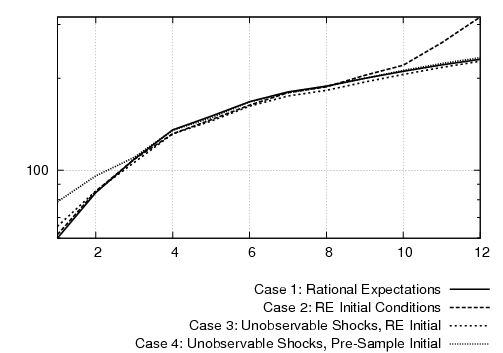
\includegraphics[scale=0.5]{consumption_fore.png} & 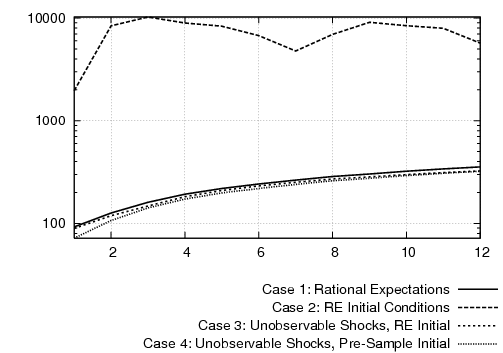
\includegraphics[scale=0.5]{investment_fore.png} \\ 
Inflation & Federal Funds Rate \\ 
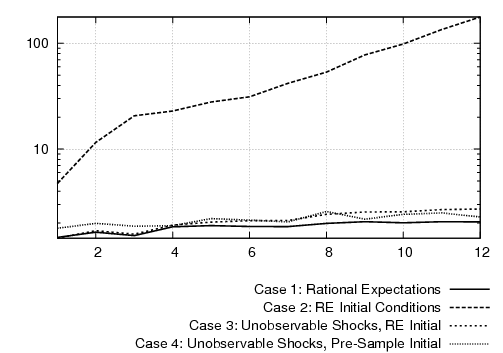
\includegraphics[scale=0.5]{inflation_fore.png} & 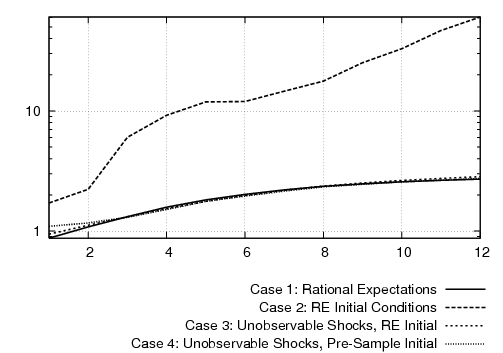
\includegraphics[scale=0.5]{fedfunds_fore.png} \\ 
\end{tabular}
\end{figure}

\begin{figure}
\caption{Preference Shock Impulse Responses}\label{fg2:irf_pref}
\vspace*{1pc}\hspace*{-0.28in}
\begin{tabular}{cccc}
\multicolumn{4}{c}{Case 1: Rational Expectations}\\
Consumption & Investment & Inflation & Interest Rate \\ 
\includegraphics[scale=0.22]{results_re/Consumption_prefshock_irf.png} & 
\includegraphics[scale=0.22]{results_re/Investment_prefshock_irf.png} & 
\includegraphics[scale=0.22]{results_re/Inflation_prefshock_irf.png} & 
\includegraphics[scale=0.22]{results_re/Interest_Rate_prefshock_irf.png} \\ \\ 
\multicolumn{4}{c}{Case 2: Learning with RE Initial Conditions}\\
Consumption & Investment & Inflation & Interest Rate \\ 
\includegraphics[scale=0.22]{results_reallinit/Consumption_prefshock_irf.png} & 
\includegraphics[scale=0.22]{results_reallinit/Investment_prefshock_irf.png} & 
\includegraphics[scale=0.22]{results_reallinit/Inflation_prefshock_irf.png} & 
\includegraphics[scale=0.22]{results_reallinit/Interest_Rate_prefshock_irf.png} \\ \\ 
\multicolumn{4}{c}{Case 3: Learning with Unobservable Shocks and RE Initial Conditions}\\
Consumption & Investment & Inflation & Interest Rate \\ 
\includegraphics[scale=0.22]{results_reinit/Consumption_prefshock_irf.png} & 
\includegraphics[scale=0.22]{results_reinit/Investment_prefshock_irf.png} & 
\includegraphics[scale=0.22]{results_reinit/Inflation_prefshock_irf.png} & 
\includegraphics[scale=0.22]{results_reinit/Interest_Rate_prefshock_irf.png} \\ \\ 
\multicolumn{4}{c}{Case 4: Learning with Unobservable Shocks and Pre-Sample Initial Conditions}\\
Consumption & Investment & Inflation & Interest Rate \\ 
\includegraphics[scale=0.22]{results_wlsinit/Consumption_prefshock_irf.png} & 
\includegraphics[scale=0.22]{results_wlsinit/Investment_prefshock_irf.png} & 
\includegraphics[scale=0.22]{results_wlsinit/Inflation_prefshock_irf.png} & 
\includegraphics[scale=0.22]{results_wlsinit/Interest_Rate_prefshock_irf.png} \\ 
\end{tabular}
\end{figure}

\begin{figure}
\caption{Technology Shock Impulse Responses}\label{fg2:irf_tech}
\vspace*{1pc}\hspace*{-0.28in}
\begin{tabular}{cccc}
\multicolumn{4}{c}{Case 1: Rational Expectations}\\
Consumption & Investment & Inflation & Interest Rate \\ 
\includegraphics[scale=0.22]{results_re/Consumption_techshock_irf.png} & 
\includegraphics[scale=0.22]{results_re/Investment_techshock_irf.png} & 
\includegraphics[scale=0.22]{results_re/Inflation_techshock_irf.png} & 
\includegraphics[scale=0.22]{results_re/Interest_Rate_techshock_irf.png} \\ \\ 
\multicolumn{4}{c}{Case 2: Learning with RE Initial Conditions}\\
Consumption & Investment & Inflation & Interest Rate \\ 
\includegraphics[scale=0.22]{results_reallinit/Consumption_techshock_irf.png} & 
\includegraphics[scale=0.22]{results_reallinit/Investment_techshock_irf.png} & 
\includegraphics[scale=0.22]{results_reallinit/Inflation_techshock_irf.png} & 
\includegraphics[scale=0.22]{results_reallinit/Interest_Rate_techshock_irf.png} \\ \\ 
\multicolumn{4}{c}{Case 3: Learning with Unobservable Shocks and RE Initial Conditions}\\
Consumption & Investment & Inflation & Interest Rate \\ 
\includegraphics[scale=0.22]{results_reinit/Consumption_techshock_irf.png} & 
\includegraphics[scale=0.22]{results_reinit/Investment_techshock_irf.png} & 
\includegraphics[scale=0.22]{results_reinit/Inflation_techshock_irf.png} & 
\includegraphics[scale=0.22]{results_reinit/Interest_Rate_techshock_irf.png} \\ \\ 
\multicolumn{4}{c}{Case 4: Learning with Unobservable Shocks and Pre-Sample Initial Conditions}\\
Consumption & Investment & Inflation & Interest Rate \\ 
\includegraphics[scale=0.22]{results_wlsinit/Consumption_techshock_irf.png} & 
\includegraphics[scale=0.22]{results_wlsinit/Investment_techshock_irf.png} & 
\includegraphics[scale=0.22]{results_wlsinit/Inflation_techshock_irf.png} & 
\includegraphics[scale=0.22]{results_wlsinit/Interest_Rate_techshock_irf.png} \\ 
\end{tabular}
\end{figure}

\begin{figure}
\caption{Investment Shock Impulse Responses}\label{fg2:irf_inv}
\vspace*{1pc}\hspace*{-0.28in}
\begin{tabular}{cccc}
\multicolumn{4}{c}{Case 1: Rational Expectations}\\
Consumption & Investment & Inflation & Interest Rate \\ 
\includegraphics[scale=0.22]{results_re/Consumption_invshock_irf.png} & 
\includegraphics[scale=0.22]{results_re/Investment_invshock_irf.png} & 
\includegraphics[scale=0.22]{results_re/Inflation_invshock_irf.png} & 
\includegraphics[scale=0.22]{results_re/Interest_Rate_invshock_irf.png} \\ \\ 
\multicolumn{4}{c}{Case 2: Learning with RE Initial Conditions}\\
Consumption & Investment & Inflation & Interest Rate \\ 
\includegraphics[scale=0.22]{results_reallinit/Consumption_invshock_irf.png} & 
\includegraphics[scale=0.22]{results_reallinit/Investment_invshock_irf.png} & 
\includegraphics[scale=0.22]{results_reallinit/Inflation_invshock_irf.png} & 
\includegraphics[scale=0.22]{results_reallinit/Interest_Rate_invshock_irf.png} \\ \\ 
\multicolumn{4}{c}{Case 3: Learning with Unobservable Shocks and RE Initial Conditions}\\
Consumption & Investment & Inflation & Interest Rate \\ 
\includegraphics[scale=0.22]{results_reinit/Consumption_invshock_irf.png} & 
\includegraphics[scale=0.22]{results_reinit/Investment_invshock_irf.png} & 
\includegraphics[scale=0.22]{results_reinit/Inflation_invshock_irf.png} & 
\includegraphics[scale=0.22]{results_reinit/Interest_Rate_invshock_irf.png} \\ \\ 
\multicolumn{4}{c}{Case 4: Learning with Unobservable Shocks and Pre-Sample Initial Conditions}\\
Consumption & Investment & Inflation & Interest Rate \\ 
\includegraphics[scale=0.22]{results_wlsinit/Consumption_invshock_irf.png} & 
\includegraphics[scale=0.22]{results_wlsinit/Investment_invshock_irf.png} & 
\includegraphics[scale=0.22]{results_wlsinit/Inflation_invshock_irf.png} & 
\includegraphics[scale=0.22]{results_wlsinit/Interest_Rate_invshock_irf.png} \\ 
\end{tabular}
\end{figure}

\begin{figure}
\caption{Monetary Policy Shock Impulse Responses}\label{fg2:irf_mp}
\vspace*{1pc}\hspace*{-0.28in}
\begin{tabular}{cccc}
\multicolumn{4}{c}{Case 1: Rational Expectations}\\
Consumption & Investment & Inflation & Interest Rate \\ 
\includegraphics[scale=0.22]{results_re/Consumption_mpshock_irf.png} & 
\includegraphics[scale=0.22]{results_re/Investment_mpshock_irf.png} & 
\includegraphics[scale=0.22]{results_re/Inflation_mpshock_irf.png} & 
\includegraphics[scale=0.22]{results_re/Interest_Rate_mpshock_irf.png} \\ \\ 
\multicolumn{4}{c}{Case 2: Learning with RE Initial Conditions}\\
Consumption & Investment & Inflation & Interest Rate \\ 
\includegraphics[scale=0.22]{results_reallinit/Consumption_mpshock_irf.png} & 
\includegraphics[scale=0.22]{results_reallinit/Investment_mpshock_irf.png} & 
\includegraphics[scale=0.22]{results_reallinit/Inflation_mpshock_irf.png} & 
\includegraphics[scale=0.22]{results_reallinit/Interest_Rate_mpshock_irf.png} \\ \\ 
\multicolumn{4}{c}{Case 3: Learning with Unobservable Shocks and RE Initial Conditions}\\
Consumption & Investment & Inflation & Interest Rate \\ 
\includegraphics[scale=0.22]{results_reinit/Consumption_mpshock_irf.png} & 
\includegraphics[scale=0.22]{results_reinit/Investment_mpshock_irf.png} & 
\includegraphics[scale=0.22]{results_reinit/Inflation_mpshock_irf.png} & 
\includegraphics[scale=0.22]{results_reinit/Interest_Rate_mpshock_irf.png} \\ \\ 
\multicolumn{4}{c}{Case 4: Learning with Unobservable Shocks and Pre-Sample Initial Conditions}\\
Consumption & Investment & Inflation & Interest Rate \\ 
\includegraphics[scale=0.22]{results_wlsinit/Consumption_mpshock_irf.png} & 
\includegraphics[scale=0.22]{results_wlsinit/Investment_mpshock_irf.png} & 
\includegraphics[scale=0.22]{results_wlsinit/Inflation_mpshock_irf.png} & 
\includegraphics[scale=0.22]{results_wlsinit/Interest_Rate_mpshock_irf.png} \\ 
\end{tabular}
\end{figure}

\begin{figure}
\caption{Smoothed Estimates of Structural Shocks}\label{fg2:shocks}
\vspace*{1pc}\hspace*{-0.28in}
\begin{tabular}{cccc}
\multicolumn{4}{c}{Case 1: Rational Expectations} \\ 
Preference & Technology & Investment & Monetary Policy \\
\includegraphics[scale=0.22]{results_re/prefshock.png} & 
\includegraphics[scale=0.22]{results_re/techshock.png} & 
\includegraphics[scale=0.22]{results_re/invshock.png} & 
\includegraphics[scale=0.22]{results_re/mpshock.png} \\ \\ 
 
\multicolumn{4}{c}{Case 2: Learning with RE Initial Conditions} \\ 
Preference (0.8708) & Technology (0.0826) & Investment (0.5076) & Monetary Policy (0.7246) \\
\includegraphics[scale=0.22]{results_reallinit/prefshock.png} & 
\includegraphics[scale=0.22]{results_reallinit/techshock.png} & 
\includegraphics[scale=0.22]{results_reallinit/invshock.png} & 
\includegraphics[scale=0.22]{results_reallinit/mpshock.png} \\ \\ 
 
\multicolumn{4}{c}{Case 3: Learning with Unobservable Shocks and RE Initial Conditions} \\ 
Preference (0.8301) & Technology (0.7917) & Investment (-0.1270) & Monetary Policy (0.2623) \\
\includegraphics[scale=0.22]{results_reinit/prefshock.png} & 
\includegraphics[scale=0.22]{results_reinit/techshock.png} & 
\includegraphics[scale=0.22]{results_reinit/invshock.png} & 
\includegraphics[scale=0.22]{results_reinit/mpshock.png} \\ \\ 
 
\multicolumn{4}{c}{Case 4: Learning with Unobservable Shocks and Pre-Sample Initial Conditions} \\ 
Preference (-0.0413) & Technology (0.7501) & Investment (-0.0976) & Monetary Policy (0.4380) \\
\includegraphics[scale=0.22]{results_wlsinit/prefshock.png} & 
\includegraphics[scale=0.22]{results_wlsinit/techshock.png} & 
\includegraphics[scale=0.22]{results_wlsinit/invshock.png} & 
\includegraphics[scale=0.22]{results_wlsinit/mpshock.png} \\ \\ 
 
\end{tabular}
\end{figure}



\end{document}



